% ==================================================================
% BÁO CÁO ĐỒ ÁN - THEO VẾT ĐA ĐỐI TƯỢNG TRONG VIDEO DRONE
% 3 detector x 5 tracker trên VisDrone2019-MOT
%
% Overleaf: Menu -> Compiler -> XeLaTeX. Chạy 2 lần để mục lục/tham chiếu đúng.
% Ảnh: tạo thư mục figures/ trên Overleaf và upload đúng tên file ghi
%      trong từng hình. Ảnh chưa có sẽ hiện khung xám ghi tên file cần upload.
%
% Giữ định dạng của khung gốc: lề trên-dưới-trái-phải = 2-2-2,5-2 cm,
% Times New Roman 13, giãn dòng 1,3, căn đều.
%
% Quy ước trình bày:
%   - Dấu phẩy thập phân xuyên suốt (51,67), kể cả trong bảng.
%   - Thuật ngữ tiếng Anh in nghiêng ở lần đầu, kèm giải thích.
%   - Tên thống nhất: YOLO11m, Faster R-CNN, RF-DETR-M, SORT, DeepSORT,
%     ByteTrack, OC-SORT, BoT-SORT.
%   - Nhận xét dưới bảng/hình: đoạn văn ngắn, lồng số vào câu, không gạch đầu dòng.
%   - Đọc HOTA trước, IDF1 sau, MOTA để tham khảo.
%
% Macro:
%   \CanDien{...}  thông tin bìa chưa được cung cấp
%   \Hinh{file}{rộng}  chèn ảnh, tự hiện khung giữ chỗ nếu chưa upload
%
% Bản khung ban đầu được giữ ở backup/bao_cao_khung_goc.tex.
% ==================================================================
\documentclass[fontsize=13pt,a4paper,oneside,parskip=false,numbers=noenddot,bibliography=totoc]{scrreprt}

% -------------------- PHÔNG CHỮ VÀ NGÔN NGỮ ----------------------
\usepackage{iftex}
\ifPDFTeX
  \usepackage[utf8]{inputenc}
  \usepackage[T5]{fontenc}
  \usepackage{mathptmx}
  \usepackage[english,main=vietnamese]{babel}
\else
  \usepackage{fontspec}
  \IfFontExistsTF{Times New Roman}
    {\setmainfont{Times New Roman}}
    {\setmainfont{TeX Gyre Termes}}   % thay thế tương đương nếu máy không có TNR
  \usepackage[english,main=vietnamese]{babel}
\fi
\usepackage{microtype}

% -------------------- KHỔ TRANG ---------------------------------
\usepackage[a4paper,top=2cm,bottom=2cm,left=2.5cm,right=2cm,
            footskip=1cm,includefoot=false]{geometry}
\usepackage{setspace}
\setstretch{1.3}                    % xấp xỉ giãn dòng 1,35 của Word
\setlength{\parindent}{1cm}
\setlength{\emergencystretch}{2em}
\usepackage{indentfirst}
\pagestyle{plain}
\raggedbottom
\setlength{\textfloatsep}{10pt plus 2pt minus 2pt}
\setlength{\intextsep}{9pt plus 2pt minus 2pt}
\renewcommand{\topfraction}{0.9}
\renewcommand{\bottomfraction}{0.8}
\renewcommand{\textfraction}{0.1}
\renewcommand{\floatpagefraction}{0.75}

% -------------------- TIÊU ĐỀ CHƯƠNG / MỤC ----------------------
\setkomafont{disposition}{\normalfont\bfseries}
\setkomafont{chapter}{\Large}
\setkomafont{section}{\large}
\setkomafont{subsection}{\normalsize}
\setkomafont{subsubsection}{\normalsize\itshape}
\RedeclareSectionCommand[beforeskip=0pt,afterskip=1\baselineskip]{chapter}
\RedeclareSectionCommand[beforeskip=-1.2\baselineskip,afterskip=0.5\baselineskip]{section}
\RedeclareSectionCommand[beforeskip=-0.9\baselineskip,afterskip=0.3\baselineskip]{subsection}
\renewcommand*{\chapterformat}{\chapapp~\thechapter.\enskip}
\setcounter{secnumdepth}{3}
\setcounter{tocdepth}{2}

% -------------------- BẢNG, HÌNH, CÔNG THỨC ---------------------
\usepackage{amsmath,amssymb,bm}
\usepackage{graphicx}
\usepackage{float}
\usepackage{booktabs}
\usepackage{tabularx}
\usepackage{multirow}
\usepackage{array}
\usepackage{etoolbox}
\AtBeginEnvironment{table}{\setstretch{1.08}}
\usepackage{subcaption}
\usepackage{caption}
\captionsetup{font=small,labelfont=bf,labelsep=period,justification=justified,singlelinecheck=true}
\captionsetup[table]{position=top,skip=4pt}
\captionsetup[figure]{skip=6pt}
\newcolumntype{C}{>{\centering\arraybackslash}X}
\newcommand{\nguon}[1]{\par\vspace{2pt}{\footnotesize\textit{#1}\par}}  % ghi chú/nguồn dưới bảng

\usepackage{eso-pic}



% -------------------- MÀU, LIÊN KẾT -----------------------------
\usepackage{xcolor}
\definecolor{goiy}{RGB}{110,110,110}
\usepackage[hidelinks,unicode]{hyperref}
\usepackage{url}
\usepackage{xurl}
\providecommand{\Repo}{\url{https://github.com/ntrThanh/uav-tracking}}

% -------------------- MACRO TIỆN ÍCH ----------------------------
\newcommand{\CanDien}[1]{{\color{goiy}\normalfont\small[#1]}}
\newlength{\HinhRong}
\newcommand{\Hinh}[2]{%
  \begingroup\setlength{\HinhRong}{#2}%
  \IfFileExists{#1}{\includegraphics[width=#2]{#1}}{%
    \fbox{\parbox[c][0.35\HinhRong][c]{\dimexpr\HinhRong-2\fboxsep-2\fboxrule}{\centering
      \color{goiy}\footnotesize Vị trí bổ sung ảnh\\\nolinkurl{#1}}}}%
  \endgroup}
\newcommand{\tm}{$\checkmark$}

\addto\captionsvietnamese{%
  \renewcommand{\contentsname}{Mục lục}%
  \renewcommand{\listfigurename}{Danh mục hình}%
  \renewcommand{\listtablename}{Danh mục bảng}%
  \renewcommand{\bibname}{Tài liệu tham khảo}%
  \renewcommand{\figurename}{Hình}%
  \renewcommand{\tablename}{Bảng}%
  \renewcommand{\appendixname}{Phụ lục}%
}

% ==================================================================
% THÔNG TIN BÁO CÁO
% ==================================================================
\newcommand{\TenTruong}{TRƯỜNG ĐẠI HỌC KHOA HỌC TỰ NHIÊN}
\newcommand{\TenKhoa}{KHOA TOÁN -- CƠ -- TIN HỌC}
\newcommand{\HocPhan}{Thị giác máy tính nâng cao}
\newcommand{\LoaiBaoCao}{BÁO CÁO ĐỒ ÁN MÔN HỌC}
\newcommand{\TenDeTai}{ỨNG DỤNG THEO VẾT ĐA ĐỐI TƯỢNG TRONG BÀI TOÁN QUẢN LÝ GIAO THÔNG}
\newcommand{\Lop}{\CanDien{K68A4}}
\newcommand{\GiangVien}{TS. Cao Văn Chung}
\newcommand{\DiaDiem}{Hà Nội}
\newcommand{\ThoiGian}{tháng 11 năm 2026}

\begin{document}

% ========================= TRANG BÌA ==============================
\hypersetup{pageanchor=false}
\newgeometry{left=2.5cm,right=2.5cm,top=3cm,bottom=3cm}
\begin{titlepage}
\AddToShipoutPictureBG*{%
  \AtPageLowerLeft{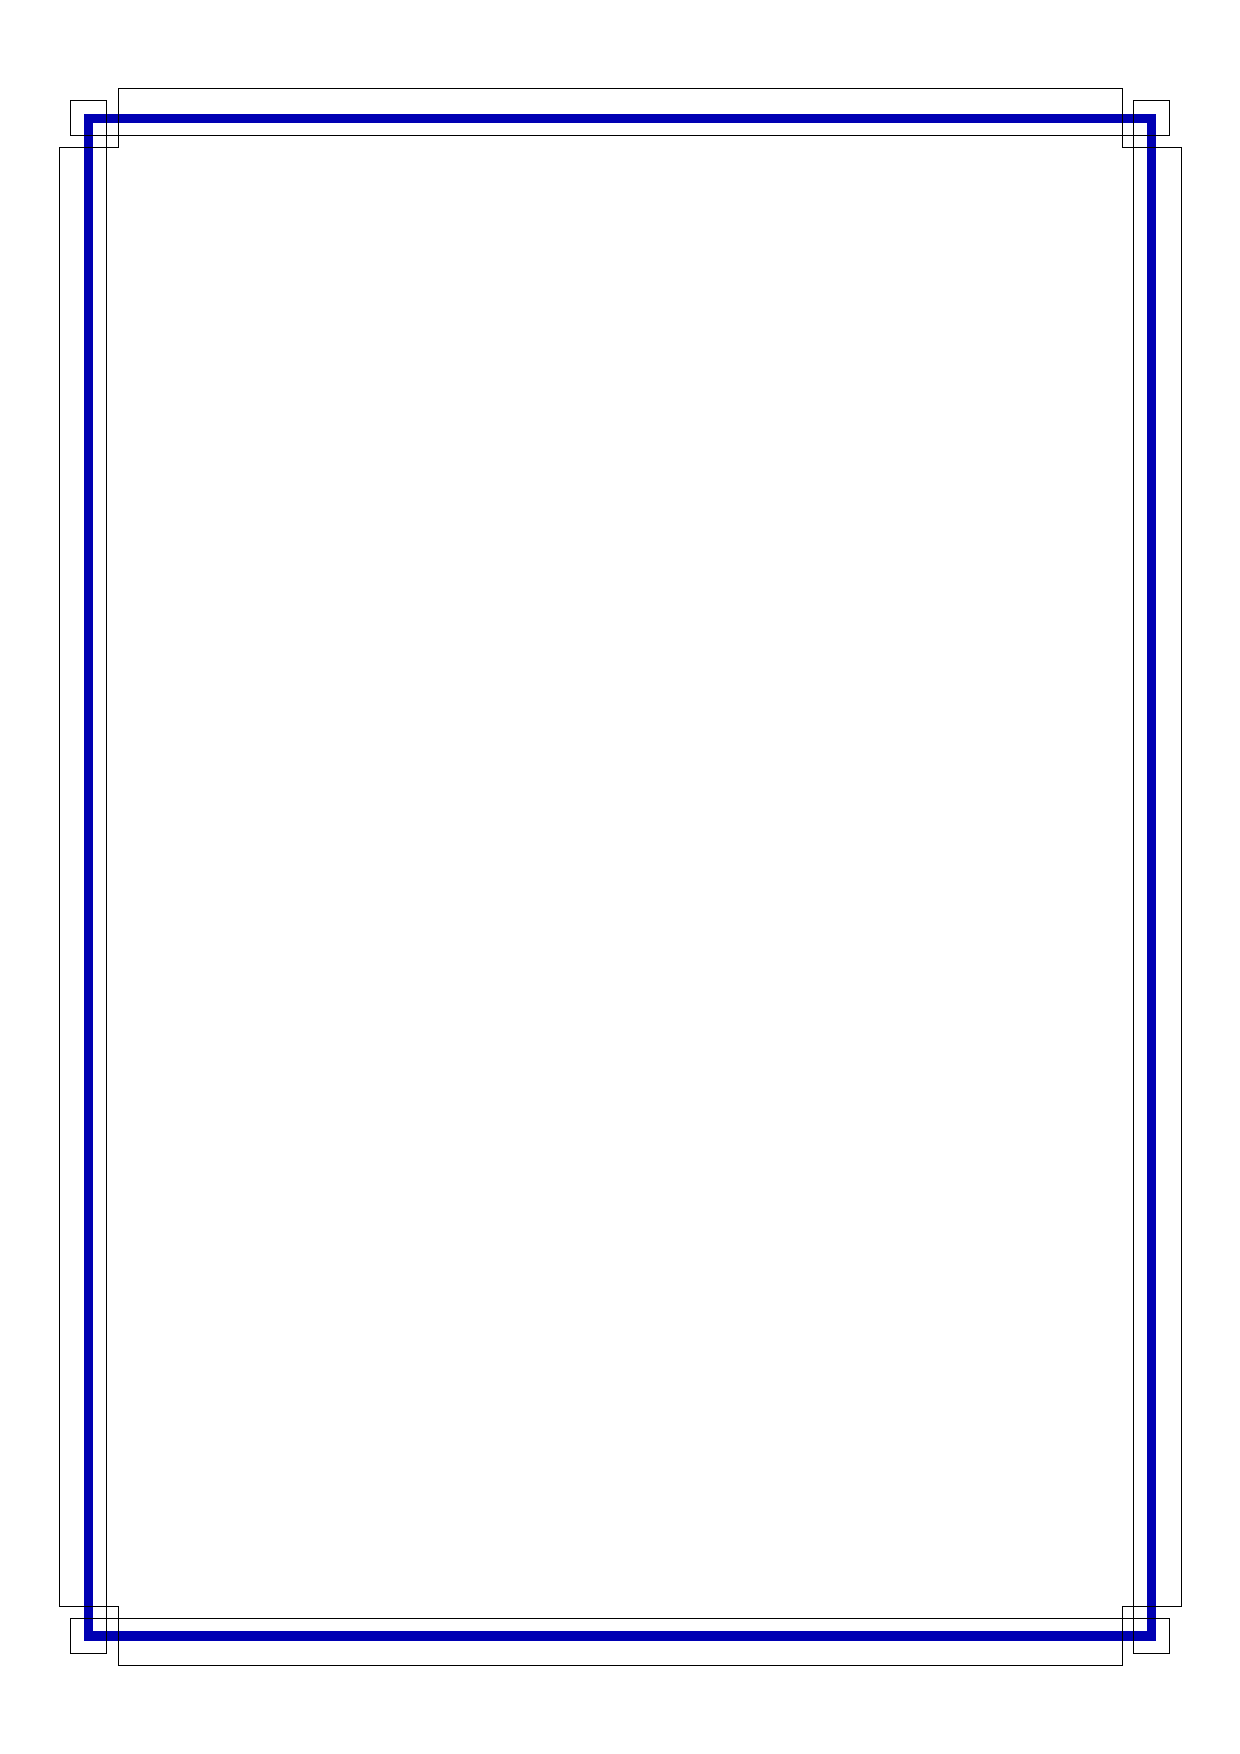
\includegraphics[width=\paperwidth,height=\paperheight]{figures/cover_border.pdf}}}
\setstretch{1.15}
\begin{center}
  {\bfseries\large ĐẠI HỌC QUỐC GIA HÀ NỘI\par}
  \vspace{0.15cm}
  {\bfseries\large \TenTruong\par}
  {\bfseries \TenKhoa\par}
  \vspace{0.55cm}
  
\includegraphics[width=4.5cm]{figures/1.png}\par
  \vspace{0.55cm}
  {\bfseries\LARGE \LoaiBaoCao\par}
  \vspace{0.3cm}
  {\large Học phần: \HocPhan\par}
  \vspace{0.85cm}
  {\bfseries\Large \TenDeTai\par}
  \vspace{1cm}
  {\large\textbf{Giảng viên hướng dẫn:} \GiangVien\par}
  \vspace{0.65cm}
  {\bfseries Nhóm sinh viên thực hiện:\par}
  \vspace{0.2cm}
  \renewcommand{\arraystretch}{1.3}
  \begin{tabular}{@{}ll@{}}
    Nguyễn Trọng Thành (nhóm trưởng) & \CanDien{23001934}\\
    Đinh Bá Thi & \CanDien{23001942}\\
    Đinh Quang Tiến & \CanDien{23001943}\\
  \end{tabular}\par
  \vspace{0.35cm}
  \textbf{Lớp:} \Lop\par
  \vspace{0.2cm}
  \vfill
  {\bfseries \DiaDiem, \ThoiGian\par}
\end{center}
\end{titlepage}
\restoregeometry
\hypersetup{pageanchor=true}

% ========================= PHẦN ĐẦU ===============================
\pagenumbering{roman}
\setcounter{page}{1}

\addchap{Tóm tắt}
% 150-250 từ, MỘT đoạn duy nhất, đủ 5 ý: bài toán, ứng dụng, dữ liệu, phương pháp, kết quả chính.
Theo vết đa đối tượng trong video từ thiết bị bay không người lái là nền tảng cho giám sát và thống kê giao thông. Góc nhìn từ trên cao, đối tượng nhỏ, che khuất và camera chuyển động làm suy giảm cả phát hiện lẫn duy trì định danh. Báo cáo khảo sát ba bộ phát hiện YOLO11m, Faster R-CNN và RF-DETR-M kết hợp năm bộ theo vết SORT, DeepSORT, ByteTrack, OC-SORT và BoT-SORT trên VisDrone2019-MOT. Các bộ phát hiện được tinh chỉnh trên VisDrone2019-DET đã loại ảnh trùng nguồn video với tập đánh giá. Mười lăm tổ hợp dùng chung bộ nhớ đệm phát hiện; ngưỡng được chọn trên tập xác thực, sau đó đánh giá trên test-dev theo năm lớp. Kết quả cho thấy BoT-SORT đạt HOTA cao nhất với cả ba bộ phát hiện, trong đó Faster R-CNN đạt 51,68 và YOLO11m đạt 51,67. Thí nghiệm dùng nhãn chuẩn thay phát hiện cho thấy khoảng cách 37,92--43,48 điểm HOTA, gợi ý phát hiện là yếu tố giới hạn chính. YOLO11m kết hợp ByteTrack đạt 101,0 khung hình/giây trong phép đo xử lý trên NVIDIA L4. Các kết quả tạo cơ sở lựa chọn cấu hình cho hệ thống giám sát giao thông thời gian thực ở cuối kỳ, hướng đến phát hiện vượt đèn đỏ và nhận dạng biển số.

\vspace{0.4cm}
\noindent\textbf{Từ khóa:} theo vết đa đối tượng, video drone, VisDrone, phát hiện đối tượng nhỏ, tracking-by-detection, HOTA.

\clearpage
\begingroup\small\setstretch{1.0}\tableofcontents\endgroup
% Bỏ comment nếu muốn có danh mục hình/bảng (tốn thêm 1-2 trang):
% \listoffigures
% \listoftables

% ========================= NỘI DUNG ===============================
\clearpage
\pagenumbering{arabic}
\setcounter{page}{1}

% ------------------------------------------------------------------
\addchap{Giới thiệu}
\label{chap:gioi-thieu}
% Khoảng 1,5 trang, 5 đoạn.

Theo vết đa đối tượng (\textit{multi-object tracking}, MOT) vừa xác định vị trí đối tượng trong từng khung hình, vừa duy trì định danh của chúng xuyên suốt video. Quỹ đạo thu được hỗ trợ đếm phương tiện, phân tích lưu lượng và phát hiện sự kiện giao thông \cite{luo2021mot}. Thiết bị bay không người lái (\textit{unmanned aerial vehicle}, UAV) mở rộng phạm vi quan sát và có thể tiếp cận nhiều khu vực mà camera cố định khó bao quát. Tuy nhiên, điều kiện thu nhận ảnh từ UAV khác đáng kể so với camera mặt đất, khiến mô hình hoạt động tốt trên dữ liệu thông thường chưa chắc giữ được chất lượng khi chuyển miền \cite{zhu2022visdrone}.

Phân tích dữ liệu VisDrone2019-MOT trong dự án cho thấy cạnh tương đương $\sqrt{wh}$ trung vị của hộp bao trên test-dev xấp xỉ 33 pixel; 47,8\% hộp có diện tích dưới $32^2$ pixel. Mỗi khung hình chứa trung bình 46,4 đối tượng và có thể lên đến 152 đối tượng. Khi ảnh tiếp tục được thu nhỏ để đưa vào mạng, nhiều đối tượng chỉ còn vài pixel. Camera chuyển động đồng thời với đối tượng còn khiến vị trí dự đoán theo mô hình vận tốc hằng dễ sai lệch. Đây là các thách thức đặc trưng của dữ liệu drone đã được đề cập trong các bộ chuẩn VisDrone và UAVDT \cite{wen2019visdronemot,du2018uavdt}.

Nhiều thuật toán MOT phổ biến được phát triển và so sánh trên dữ liệu người đi bộ từ camera mặt đất như MOT16/17 và MOT20 \cite{milan2016mot16,dendorfer2020mot20}. Những bộ dữ liệu này gồm các điều kiện camera khác nhau, nhưng chưa phản ánh đầy đủ góc nhìn trên cao và mật độ vật thể nhỏ của VisDrone. Vì vậy, cần đánh giá lại cả bộ phát hiện (\textit{detector}) và bộ theo vết (\textit{tracker}) trong cùng điều kiện, đồng thời phân biệt lỗi bỏ sót đối tượng với lỗi liên kết định danh.

Báo cáo tập trung trả lời ba câu hỏi. Thứ nhất, với một giao thức thống nhất, tổ hợp detector và tracker nào cho chất lượng theo vết tốt nhất (Q1)? Thứ hai, khâu phát hiện hay khâu liên kết là yếu tố giới hạn chính của hệ thống (Q2)? Thứ ba, cấu hình nào tạo được đánh đổi phù hợp giữa chất lượng và tốc độ để phát triển ứng dụng thực tế (Q3)? Phạm vi thực nghiệm hiện tại là phát hiện và theo vết trên dữ liệu có sẵn; mục tiêu cuối kỳ là tích hợp nền tảng này thành hệ thống giám sát giao thông thời gian thực, bổ sung phát hiện vượt đèn đỏ, phát hiện biển số và nhận dạng ký tự biển số.

Đóng góp của nhóm là xây dựng quy trình tiền xử lý và đánh giá dùng chung, tổng hợp ma trận 15 tổ hợp và thực hiện thí nghiệm \textit{oracle}, tức thay đầu ra detector bằng nhãn chuẩn để khảo sát tracker khi phát hiện lý tưởng. Phân tích tách độ chính xác phát hiện DetA và độ chính xác liên kết AssA giúp giải thích kết quả thay vì chỉ xếp hạng theo một điểm tổng. Chương~\ref{chap:phuong-phap} trình bày phương pháp và dữ liệu; Chương~\ref{chap:thuc-nghiem} trình bày thực nghiệm, phân tích và giới hạn. Phần kết luận xác định hướng tích hợp cho đồ án cuối kỳ.



% ------------------------------------------------------------------
\chapter{Phương pháp và dữ liệu}
\label{chap:phuong-phap}

\section{Phương pháp}
\label{sec:phuong-phap}

\subsection{Pipeline tổng thể}
\label{sec:pipeline}

Hình~\ref{fig:pipeline} mô tả quy trình theo vết dựa trên phát hiện (\textit{tracking-by-detection}). Detector xử lý các khung hình và ghi bộ nhớ đệm phát hiện (\textit{DET cache}) ở ngưỡng điểm tin cậy 0,05. Mỗi phát hiện gồm chỉ số khung hình, tọa độ hộp bao trên ảnh gốc, điểm tin cậy và lớp đối tượng theo VisDrone. Với mỗi detector, cả năm tracker đọc cùng cache, qua đó loại bỏ sai khác do chạy lại suy luận. So sánh giữa các tracker còn bao gồm ngưỡng riêng được chọn bằng cùng tiêu chí trên val.

Hệ thống chỉ đưa năm lớp đánh giá vào tracker và ghép cặp trong từng lớp. Mỗi khung hình trải qua dự đoán chuyển động, bù chuyển động camera hoặc trích đặc trưng ngoại hình nếu thuật toán có sử dụng, ghép cặp và cập nhật vòng đời quỹ đạo. Kết quả được lọc theo vùng không đánh giá (\textit{ignored region}) trước khi chuyển cho TrackEval. Nhánh oracle dùng hộp nhãn chuẩn với score bằng 1 nhưng không cung cấp ID chuẩn cho tracker; tracker vẫn phải tự liên kết các hộp qua thời gian.

\begin{figure}[!htbp]
  \centering
  \resizebox{\linewidth}{!}{%
  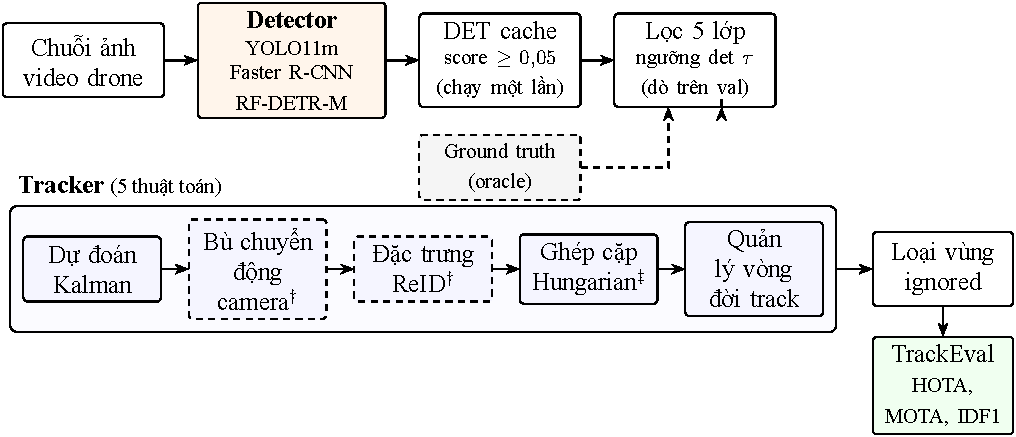
\includegraphics{figures/pipeline_vector.pdf}}
  \caption{Pipeline tổng thể với DET cache dùng chung. Trong cùng detector, các tracker nhận cùng nguồn phát hiện và dùng ngưỡng chọn trên val. Nhánh nét đứt thay phát hiện bằng nhãn chuẩn. $^{\dagger}$Khối tùy chọn: ReID ở DeepSORT và BoT-SORT; bù chuyển động camera (GMC) ở BoT-SORT. $^{\ddagger}$ByteTrack và BoT-SORT ghép hai tầng theo score.}
  \label{fig:pipeline}
\end{figure}

\subsection{Ba detector}
\label{sec:detector}

Ba detector đại diện cho ba hướng thiết kế: Faster R-CNN dùng hai giai đoạn, YOLO11m dùng một giai đoạn và RF-DETR-M dùng transformer dự đoán tập đối tượng. Cả ba được khởi tạo từ trọng số tiền huấn luyện trên COCO và tinh chỉnh trên cùng tập DET đã làm sạch. Bảng~\ref{tab:detector} trình bày cấu hình được dùng thực tế; đây là so sánh giữa các cấu hình triển khai, không phải phép thử giữ nguyên độ phân giải để chỉ đo ảnh hưởng kiến trúc.

\begin{table}[!htbp]
  \centering
  \caption{So sánh kiến trúc và chi phí tính toán của ba detector}
  \label{tab:detector}
  \small
  \begin{tabularx}{\textwidth}{@{}lCCC@{}}
    \toprule
    & \textbf{Faster R-CNN} & \textbf{YOLO11m} & \textbf{RF-DETR-M}\\
    \midrule
    Họ kiến trúc & Hai giai đoạn & Một giai đoạn & Transformer end-to-end\\
    Backbone & ResNet-50 + FPN & CSP (C3k2, C2PSA) & ViT với tiền huấn luyện DINOv2\\
    Kích thước ảnh vào & 800--1333 & 640 & 576\\
    Cần NMS & Có & Có & Không\\
    Số tham số (M) & 43,3 & 20,1 & 33,4\\
    GFLOPs / frame & 745,5 & 40,7 & 78,4\\
    FPS detector & 13,8 & 118,3 & 32,8\\
    \bottomrule
  \end{tabularx}
  \nguon{GFLOPs được tính với quy ước 2 FLOPs/phép nhân-cộng, trung bình có trọng số theo độ phân giải ảnh; không lấy từ benchmark nhà phát triển. FPS trên một NVIDIA L4, batch 1, 905 frame test-dev.}
\end{table}

\subsubsection{Faster R-CNN R50-FPN v2}
Faster R-CNN trước tiên dùng mạng đề xuất vùng (RPN) để sinh các vùng có khả năng chứa đối tượng, sau đó phân loại và hồi quy hộp bao tại đầu RoI \cite{ren2015faster}. Mạng tháp đặc trưng (FPN) kết hợp các mức đặc trưng để xử lý nhiều kích thước đối tượng \cite{lin2017fpn}. Dự án dùng bản Faster R-CNN ResNet-50 FPN v2 của torchvision \cite{li2021benchmarking}, thay đầu phân loại thành 11 đầu ra gồm nền và 10 lớp. Ảnh được giữ tỉ lệ, đưa cạnh ngắn về 800 pixel và chặn cạnh dài ở 1.333 pixel. Độ phân giải này có thể giữ nhiều chi tiết cho đối tượng nhỏ, nhưng làm tăng chi phí tính toán.

RPN dự đoán điểm có đối tượng và độ lệch của hộp so với anchor; đầu RoI tiếp tục phân loại và tinh chỉnh các vùng đề xuất. Tổng mất mát có bốn thành phần: phân loại và hồi quy ở RPN, phân loại và hồi quy ở RoI. Bản torchvision hiện đại sử dụng FPN và RoIAlign; các thành phần này cần được phân biệt với thiết kế VGG16/RoI Pool trong nghiên cứu Faster R-CNN ban đầu.

\subsubsection{YOLO11m}
YOLO dự đoán vị trí và lớp đối tượng trực tiếp từ các bản đồ đặc trưng trong một lượt xử lý \cite{redmon2016yolo}. Biến thể YOLO11m dùng các khối C3k2, C2PSA và đặc trưng đa mức để cân bằng biểu diễn với chi phí suy luận \cite{jocher2024yolo11,khanam2024yolov11}. Ảnh được đệm giữ tỉ lệ về kích thước 640; bước loại cực đại không gian (\textit{non-maximum suppression}, NMS) khử hộp trùng với ngưỡng IoU 0,7. Khi lưu cache, mô hình cho phép tối đa 1.000 hộp mỗi ảnh. Cấu hình này ưu tiên thông lượng, song việc thu nhỏ ảnh có thể làm mất tín hiệu của các đối tượng rất nhỏ.

Trong cấu hình detection chuẩn, neck kết hợp đường truyền đặc trưng từ trên xuống và từ dưới lên; head dự đoán tại ba mức stride 8, 16 và 32. Head không dùng các hộp anchor kích thước định trước, mà dự đoán phân phối khoảng cách từ điểm lưới đến bốn cạnh hộp. Hàm mất mát gồm thành phần định vị dựa trên IoU, phân loại và Distribution Focal Loss (DFL); cơ chế gán mẫu dương xét đồng thời điểm lớp với chất lượng hộp. 

\subsubsection{RF-DETR-M}
RF-DETR kế thừa hướng dự đoán tập đối tượng của DETR, Deformable DETR và LW-DETR \cite{carion2020detr,zhu2021deformable,chen2024lwdetr}. Mô hình dùng backbone thị giác transformer với tiền huấn luyện DINOv2 \cite{oquab2024dinov2} và các truy vấn đối tượng (\textit{object query}); cấu hình Medium trong dự án suy luận ở 576 pixel và giới hạn 300 phát hiện. Ghép cặp một-một trong huấn luyện giảm nhu cầu dùng NMS ở đầu ra \cite{robinson2025rfdetr}. Với patch 16 pixel, các đối tượng chỉ còn vài pixel sau resize có ít thông tin để biểu diễn. Đây là giả thuyết cần đối chiếu bằng AP theo kích thước, không phải khẳng định rằng mạng không thể phát hiện đối tượng nhỏ hơn một patch.

Đặc trưng ViT được đưa qua bộ chiếu đặc trưng, rồi decoder dùng các query và điểm tham chiếu không gian để lấy thông tin bằng deformable cross-attention. Query là vị trí dự đoán trong biểu diễn học được, khác với vùng RoI được cắt từ đặc trưng của Faster R-CNN. Mất mát dự đoán tập kết hợp phân loại, khoảng cách $L_1$ giữa hộp và GIoU sau ghép cặp, cùng giám sát ở các tầng trung gian. Paper RF-DETR còn đề xuất tìm kiếm kiến trúc dùng chung trọng số (NAS) để lựa chọn đánh đổi độ trễ--độ chính xác \cite{robinson2025rfdetr}. Trong đồ án, nhóm tinh chỉnh cấu hình Medium có sẵn, không chạy lại toàn bộ NAS. Các query ở mỗi frame cũng không phải ID ổn định theo thời gian; RF-DETR vẫn cần tracker bên ngoài.

\subsection{Năm tracker}
\label{sec:tracker}

Các tracker trong báo cáo đều theo mô hình \textit{tracking-by-detection} (theo vết dựa trên phát hiện) và chia sẻ hai thành phần chung. Thứ nhất là bộ lọc Kalman \cite{kalman1960} với mô hình vận tốc hằng. SORT dùng vector trạng thái
\begin{equation}
  \mathbf{x} = [u, v, s, r, \dot u, \dot v, \dot s]^\top,
  \label{eq:state-sort}
\end{equation}
trong đó $(u,v)$ là tâm box, $s$ là diện tích và $r$ là tỉ lệ cạnh. BoT-SORT dùng trạng thái tám chiều gồm tâm, chiều rộng, chiều cao và bốn thành phần vận tốc tương ứng. Bước dự đoán là
\begin{equation}
  \hat{\mathbf{x}}_{t|t-1} = \mathbf{F}\,\mathbf{x}_{t-1}, \qquad
  \mathbf{P}_{t|t-1} = \mathbf{F}\,\mathbf{P}_{t-1}\mathbf{F}^\top + \mathbf{Q}.
  \label{eq:kalman}
\end{equation}
Thứ hai là ghép cặp giữa quỹ đạo dự đoán $\hat b_i$ và detection $d_j$ bằng thuật toán Hungarian \cite{kuhn1955} trên ma trận chi phí
\begin{equation}
  C_{ij} = 1 - \mathrm{IoU}(\hat b_i, d_j).
  \label{eq:iou-cost}
\end{equation}

\textbf{SORT} \cite{bewley2016sort} là mốc cơ sở, sử dụng Kalman, IoU và Hungarian. Detection chưa ghép được tạo quỹ đạo mới; quỹ đạo mất quan sát quá thời gian mất dấu cho phép bị xóa. Cách làm đơn giản và nhanh nhưng dễ đổi ID khi các đối tượng giao nhau hoặc bị che khuất.

\textbf{DeepSORT} \cite{wojke2017deepsort} bổ sung đặc trưng tái định danh (\textit{re-identification}, ReID). Khoảng cách cosine giữa đặc trưng detection và bộ nhớ ngoại hình của quỹ đạo được kết hợp với ràng buộc chuyển động Mahalanobis. Cơ chế ghép theo tầng ưu tiên quỹ đạo được quan sát gần nhất, rồi ghép bằng IoU cho các trường hợp còn lại. Hiệu quả phụ thuộc mức phù hợp của mạng ReID với góc nhìn và kích thước đối tượng.

\textbf{ByteTrack} \cite{zhang2022bytetrack} khai thác các phát hiện có điểm tin cậy thấp. Sau khi ghép quỹ đạo với nhóm score cao, thuật toán ghép những quỹ đạo còn lại với nhóm score thấp bằng IoU. Nhờ vậy, một đối tượng tạm thời mờ hoặc bị che vẫn có cơ hội giữ ID. Nhóm score thấp không được dùng để khởi tạo quỹ đạo mới, nhằm hạn chế quỹ đạo giả.

\textbf{OC-SORT} \cite{cao2023ocsort} lấy quan sát làm trung tâm để hạn chế sai lệch tích lũy của Kalman. Cơ chế OCM đưa hướng chuyển động từ các quan sát vào chi phí ghép; OCR thử khôi phục liên kết bằng hộp quan sát gần nhất; ORU cập nhật lại bộ lọc qua các quan sát ảo khi tìm lại đối tượng sau một khoảng mất dấu. Các cơ chế này cần quan sát đủ tin cậy để ước lượng chuyển động.

\textbf{BoT-SORT} \cite{aharon2022botsort} mở rộng ghép hai tầng của ByteTrack với trạng thái Kalman theo chiều rộng và chiều cao, ReID và bù chuyển động camera (\textit{global motion compensation}, GMC). Trong thực nghiệm, BoT-SORT dùng luồng quang học thưa \cite{lucas1981,shi1994} để ước lượng biến đổi camera, sau đó hiệu chỉnh trạng thái và hiệp phương sai trước khi ghép. Cấu hình thực nghiệm bật cả GMC và ReID.

Với BoT-SORT, gọi $s_j$ là score của detection, $d^{\mathrm{IoU}}_{ij}=1-\mathrm{IoU}_{ij}$ và $d^{\cos}_{ij}$ là khoảng cách cosine. Chi phí hình học có kết hợp score là $d^{\mathrm{fused}}_{ij}=1-\mathrm{IoU}_{ij}s_j$. Khoảng cách ngoại hình sau khi chia đôi được chặn bởi ngưỡng ngoại hình và ngưỡng gần nhau:
\begin{equation}
  \hat d^{\cos}_{ij} =
  \begin{cases}
    0{,}5\, d^{\cos}_{ij}, & 0{,}5d^{\cos}_{ij} \leq \theta_{\mathrm{emb}} \ \text{và}\ d^{\mathrm{IoU}}_{ij} \leq \theta_{\mathrm{IoU}},\\
    1, & \text{ngược lại},
  \end{cases}
  \qquad
  C_{ij} = \min\bigl(d^{\mathrm{fused}}_{ij},\, \hat d^{\cos}_{ij}\bigr).
  \label{eq:botsort-cost}
\end{equation}

Bảng~\ref{tab:tracker-thanh-phan} tóm tắt thành phần của từng tracker. DeepSORT và BoT-SORT dùng chung trọng số ReID OSNet-x0.25 huấn luyện trên MSMT17 \cite{zhou2019osnet,wei2018msmt17}. Năm tracker sử dụng thống nhất các thành phần biểu diễn quỹ đạo, dự đoán chuyển động và ghép cặp trong cùng quy trình đánh giá.

\begin{table}[!htbp]
  \centering
  \caption{Thành phần của năm tracker}
  \label{tab:tracker-thanh-phan}
  \small
  \begin{tabularx}{\textwidth}{@{}lcccc>{\raggedright\arraybackslash}X@{}}
    \toprule
    \textbf{Tracker} & \textbf{Kalman} & \shortstack{\textbf{Ghép hai}\\\textbf{tầng}} & \textbf{ReID} & \textbf{GMC} & \textbf{Điểm đặc trưng}\\
    \midrule
    SORT      & \tm & & & & Mốc: Kalman + IoU + Hungarian\\
    DeepSORT  & \tm & & \tm & & Khoảng cách cosine, matching cascade\\
    ByteTrack & \tm & \tm & & & Tận dụng box score thấp ở tầng hai\\
    OC-SORT   & \tm & & & & Lấy quan sát làm trung tâm (ORU, OCM, OCR)\\
    BoT-SORT  & \tm & \tm & \tm & \tm & ByteTrack + ReID + bù chuyển động camera\\
    \bottomrule
  \end{tabularx}
\end{table}

\subsection{Thuật toán theo vết tổng quát}
\label{sec:pseudo}

Quy trình theo vết xử lý tuần tự từng khung hình: dự đoán vị trí quỹ đạo, ghép với các phát hiện, cập nhật trạng thái và quản lý quỹ đạo mới hoặc mất dấu. Chi phí ghép và điều kiện xuất quỹ đạo được thay theo từng tracker; DeepSORT dùng ghép theo tầng và OC-SORT bổ sung cập nhật dựa trên quan sát. Trạng thái được khởi tạo lại khi đổi video, còn khung hình không có detection vẫn phải được xử lý để cập nhật tuổi quỹ đạo. Bộ lọc đầu vào phải giữ nhóm score thấp cho ByteTrack và BoT-SORT.



% ------------------------------------------------------------------
\section{Dữ liệu và tiền xử lý}
\label{sec:du-lieu}

\subsection{Nguồn dữ liệu và phân chia}

Dữ liệu lấy từ VisDrone2019-MOT và VisDrone2019-DET, được thu nhận bằng drone tại nhiều thành phố của Trung Quốc \cite{zhu2022visdrone,wen2019visdronemot}. MOT cung cấp chuỗi khung hình và ID đối tượng; DET cung cấp ảnh tĩnh với hộp bao. Các chuỗi có độ phân giải khác nhau, từ $680\times382$ đến $3840\times2160$ pixel trong bộ dữ liệu. Bảng~\ref{tab:du-lieu} thống kê MOT trước bước lọc vùng ignored.

Ba detector của ma trận chính được huấn luyện trên 6.414 ảnh DET train sau khi loại 57 ảnh trùng nguồn video với MOT val/test-dev. Tập DET val gồm 548 ảnh dùng để chọn checkpoint; tập MOT val gồm 2.846 khung hình dùng để chọn ngưỡng tracker. Tập MOT test-dev gồm 6.635 khung hình dùng để báo cáo kết quả theo vết sau khi khóa cấu hình. DET test-dev có 1.610 ảnh và chỉ xuất hiện trong thí nghiệm detection bổ trợ, không được đồng nhất với MOT test-dev. Dữ liệu MOT train ở bảng dưới phục vụ EDA và thí nghiệm chẩn đoán nguồn huấn luyện.

\begin{table}[!htbp]
  \centering
  \caption{Thống kê và vai trò của các tập dữ liệu}
  \label{tab:du-lieu}
  \small
  \setlength{\tabcolsep}{4pt}
  \begin{tabularx}{\textwidth}{@{}lrrrrrrX@{}}
    \toprule
    \textbf{Tập} & \textbf{Chuỗi} & \textbf{Frame} & \textbf{Box} & \textbf{Quỹ đạo} & \textbf{Box/frame} & \textbf{Small (\%)} & \textbf{Vai trò}\\
    \midrule
    MOT train    & 56 & 24.201 & 1.105.516 & 7.342 & 45,7 & 24,9 & EDA, chẩn đoán\\
    MOT val      & 7  & 2.846  & 114.132   & 758   & 40,1 & 19,2 & Dò ngưỡng\\
    MOT test-dev & 17 & 6.635  & 307.799   & 2.293 & 46,4 & 47,8 & Đánh giá\\
    \bottomrule
  \end{tabularx}
  \nguon{Box tính trên 10 lớp. Small: box có diện tích nhỏ hơn $32^2$ px. }
\end{table}

\subsection{Quy ước nhãn}
Nhãn VisDrone gồm 12 mã từ 0 đến 11. Mã 0 biểu thị vùng ignored; mã 11 là nhóm \textit{others} và bị loại khỏi tập lớp mục tiêu. Detector được huấn luyện trên 10 lớp từ 1 đến 10. Đánh giá tracking giới hạn ở năm lớp pedestrian, car, van, truck và bus; các lớp này được đánh dấu trong Bảng~\ref{tab:det-lop}. Hộp bao dùng góc trên trái $(x,y)$ cùng chiều rộng $w$ và chiều cao $h$. Nhãn MOT bổ sung frame và ID; các trường truncation và occlusion mô tả mức cắt biên và che khuất. Score trong nhãn chuẩn là cờ đánh giá, khác với xác suất dự đoán của detector. Mã lớp nội bộ 0--9 của YOLO11m và RF-DETR-M được cộng 1 khi xuất cache; Faster R-CNN giữ mã 1--10, với mã 0 dành cho nền.

\subsection{Phân tích dữ liệu}

Hình~\ref{fig:eda} cho thấy dữ liệu mất cân bằng cả về lớp và kích thước. Trên train, tỉ lệ số hộp giữa lớp nhiều nhất và ít nhất xấp xỉ 52 lần. Đối tượng nhỏ chiếm 24,9\% trên train, 19,2\% trên val nhưng 47,8\% trên test-dev, gần gấp đôi train. Mật độ trung bình từ 40,1 đến 46,4 hộp mỗi khung hình gây nhiều tình huống che khuất và giao cắt. Khi quy đổi ảnh về 576 pixel, thống kê EDA ghi nhận 24,3\% hộp test-dev có cạnh ngắn dưới 8 pixel; ở 1.024 pixel, tỉ lệ này còn 4,7\%. Sự khác biệt kích thước giữa các tập là một yếu tố cần xét khi diễn giải hiệu quả tổng quát hóa ở mục~\ref{sec:phan-tich}.

\begin{figure}[!htbp]
  \centering
  \begin{subfigure}[t]{0.95\linewidth}\centering
    \Hinh{figures/05_class_distribution.png}{\linewidth}\caption{Phân bố số lượng nhãn theo 10 lớp: Lớp xe con (car) và người đi bộ (pedestrian) chiếm tỉ trọng áp đảo; các lớp xe ba bánh (tricycle, awning-tricycle) chiếm tỉ lệ rất nhỏ, thể hiện độ mất cân bằng lớp nghiêm trọng.}\end{subfigure}\hfill
  \par\smallskip
  \begin{subfigure}[t]{0.95\linewidth}\centering
    \Hinh{figures/06_box_size.png}{\linewidth}\caption{Tỉ lệ diện tích hộp bao (bounding box) theo ba nhóm chuẩn COCO: Nhỏ ($S < 32^2$), Vừa ($32^2 \le M \le 96^2$) và Lớn ($L > 96^2$ px). Tập test-dev có tỷ lệ vật thể siêu nhỏ lên tới 47,8\%, gần gấp đôi tập train (24,9\%) và val (19,2\%).}\end{subfigure}\hfill
  \par\smallskip
  \begin{subfigure}[t]{0.7\linewidth}\centering
    \Hinh{figures/08_density.png}{\linewidth}\caption{Phân bố mật độ đối tượng trên mỗi khung hình: Tập trung chủ yếu từ 40 đến 80 đối tượng/frame, tạo nên mật độ giao thông dày đặc và làm tăng tần suất giao cắt, che khuất.}\end{subfigure}
  \caption{Đặc trưng phân bố không gian và thuộc tính nhãn trên tập dữ liệu VisDrone2019-MOT qua phân tích khám phá dữ liệu (EDA). Bộ dữ liệu thể hiện rõ tính chất bất cân xứng về phân bố lớp, độ áp đảo của đối tượng kích thước siêu nhỏ ở góc nhìn UAV trên tập kiểm thử test-dev, và mật độ giao thông đông đúc.}
  \label{fig:eda}
\end{figure}

\subsection{Chiến lược lấy mẫu và làm sạch}
Quy trình tiền xử lý thống nhất cách đọc nhãn, cắt hộp về biên ảnh, bỏ hộp có cạnh dưới 1 pixel và xuất COCO, YOLO, RF-DETR cùng MOTChallenge. Vùng ignored được lưu riêng để dùng khi đánh giá; ảnh không bị tô đen ở các vùng này. Với biến thể huấn luyện bằng MOT, nhóm lấy một trong hai frame liên tiếp (stride 2), còn val/test-dev giữ đầy đủ. Các định dạng được kiểm tra chéo về số ảnh, số hộp, mã lớp và tọa độ trước khi huấn luyện. Biến thể DET dùng toàn bộ ảnh còn lại sau làm sạch, không áp dụng stride 2.

Để hạn chế rò rỉ dữ liệu, nhóm loại các ảnh DET có cùng mã video với MOT val/test-dev khỏi tập huấn luyện. Có 45 ảnh trùng nguồn với val và 12 ảnh trùng nguồn với test-dev, tổng cộng 57 ảnh. Danh sách ảnh huấn luyện DET còn 6.414 ảnh. Việc giữ nguyên phân chia theo chuỗi tránh đưa các frame gần trùng của một video vào cả tập học và tập đánh giá.

Thí nghiệm chẩn đoán RF-DETR-M trong Bảng~\ref{tab:nguon-train} cho thấy nguy cơ quá khớp theo cảnh: với nguồn MOT, mAP train tăng từ 39,12 lên 58,02 trong khi mAP val giảm từ 23,32 xuống 17,79 giữa epoch 1 và 16. Dù số frame lớn, chúng chỉ thuộc 56 chuỗi và có mức dư thừa thời gian cao. Nhóm vì vậy chọn nguồn DET cho cả ba detector để tăng sự đa dạng ảnh huấn luyện. Trên tập con MOT của phép chẩn đoán, checkpoint học từ DET đạt mAP test-dev 22,38 so với 19,78 của checkpoint MOT epoch 1. Tuy nhiên, AP nhỏ lại giảm từ 9,07 xuống 7,99; thay nguồn học không giải quyết đồng thời mọi nhóm kích thước. Các số này chỉ so sánh trong giao thức chẩn đoán, không thay thế đánh giá đầy đủ ở Chương~\ref{chap:thuc-nghiem}.

\begin{table}[!htbp]
  \centering
  \caption{Ảnh hưởng của nguồn dữ liệu huấn luyện đến RF-DETR-M (mAP50-95, \%)}
  \label{tab:nguon-train}
  \small
  \begin{tabularx}{\textwidth}{@{}lXrrrr@{}}
    \toprule
    \textbf{Nguồn train} & \textbf{Checkpoint} & \textbf{Train} & \textbf{Val} & \textbf{Test-dev} & \textbf{AP\textsubscript{S} test-dev}\\
    \midrule
    Frame MOT & Epoch 1 (tốt nhất trên val) & 39,12 & 23,32 & 19,78 & 9,07\\
    Frame MOT & Epoch 16 (cuối)             & 58,02 & 17,79 & 17,80 & 6,14\\
    Ảnh DET   & Tốt nhất trên val           & 22,49 & 22,13 & 22,38 & 7,99\\
    \bottomrule
  \end{tabularx}
  \nguon{Đánh giá bổ trợ trên tập con frame MOT (train 1.238 frame, test-dev 1.332 frame), không so sánh trực tiếp với Bảng~\ref{tab:det}. }
\end{table}

% ------------------------------------------------------------------
\chapter{Thực nghiệm và đánh giá}
\label{chap:thuc-nghiem}

\section{Thiết lập thực nghiệm}
\label{sec:thiet-lap}

\subsection{Môi trường và cấu hình huấn luyện}
YOLO11m chạy trên Tesla T4 với PyTorch 2.11.0 (CUDA 12.8) và Ultralytics 8.4.197; Faster R-CNN chạy trên NVIDIA L4 với PyTorch 2.11.0 (CUDA 13.0) và torchvision 0.26.0 (CUDA 13.0). RF-DETR-M dùng hai NVIDIA L4, thư viện RF-DETR 1.11.2. Bảng~\ref{tab:hyper} trình bày cấu hình huấn luyện trên DET. RF-DETR-M được huấn luyện tối đa 40 epoch với batch 8 mỗi GPU, không tích lũy gradient.

Phép đo tốc độ được thực hiện riêng trên một NVIDIA L4, batch 1, FP32, cùng 905 frame thuộc ba chuỗi test-dev có mật độ khác nhau. Detector khởi động bằng 50 frame, đồng bộ CUDA trước và sau mỗi lần suy luận; ba lượt đo được tổng hợp bằng trung vị. Môi trường đo tốc độ sử dụng Python 3.11.17 và PyTorch 2.15.0+cu132. Tracker cũng có lượt khởi động trước ba lượt đo. Thời gian đọc/giải mã ảnh, ghi kết quả và hiển thị không nằm trong các bộ đếm xử lý; tốc độ toàn ứng dụng phải đo lại khi triển khai.

\begin{table}[!htbp]
  \centering
  \caption{Siêu tham số huấn luyện ba detector}
  \label{tab:hyper}
  \small
  \begin{tabularx}{\textwidth}{@{}lXXX@{}}
    \toprule
    & \textbf{Faster R-CNN} & \textbf{YOLO11m} & \textbf{RF-DETR-M}\\
    \midrule
    Ảnh vào & 800--1333 & 640 & 576\\
    Số epoch & 24; giảm lr sau epoch 16 và 22 & 80; tắt mosaic 10 epoch cuối; patience 20 & Tối đa 40; dừng sớm với patience 8\\
    Optimizer & SGD, lr $0{,}02\times$batch/16, momentum 0,9 & SGD, lr 0,01, cosine, warmup 3 epoch & AdamW, lr $10^{-4}$, lr encoder $1{,}5\times10^{-4}$\\
    Weight decay & $10^{-4}$ & $5\times10^{-4}$ & $10^{-4}$\\
    Batch & 4 & 16 & $8\times2$ GPU, không tích lũy\\
    Chọn checkpoint & mAP DET val cao nhất, epoch 17 & mAP DET val cao nhất, epoch 60 & \textit{best\_total} trên DET val\\
    \bottomrule
  \end{tabularx}
  \nguon{Seed 0 cho cả ba. AMP được ghi bật trong cấu hình YOLO11m và Faster R-CNN; RF-DETR dùng thiết lập thư viện. Chưa xác định epoch tốt nhất của RF-DETR-M trong phạm vi thống kê này.}
\end{table}

\subsection{Kịch bản thực nghiệm}
Thực nghiệm gồm bốn giai đoạn. E0 đánh giá chất lượng phát hiện của ba detector trên cùng cache và bộ nhãn MOT. E1 chạy ma trận 15 tổ hợp với tham số mặc định trong Bảng~\ref{tab:tracker-param}. E2 dò ngưỡng cao $\tau\in\{0{,}3;0{,}4;\ldots;0{,}8\}$ cho từng cặp detector--tracker trên MOT val, chọn HOTA cao nhất và dùng cấu hình đó để lập bảng chính trên MOT test-dev. E3 thay detection bằng nhãn chuẩn và chạy năm tracker để phân tích khoảng cách oracle. Checkpoint được chọn trên DET val, ngưỡng tracker được chọn trên MOT val; test-dev dùng để báo cáo, không làm tiêu chí chọn tham số.

Với ByteTrack và BoT-SORT, cấu hình giữ ngưỡng thấp 0,1 và điều chỉnh ngưỡng tạo track mới cùng ngưỡng cao theo $\tau_{\mathrm{new}}=\max(\tau,\min(\tau+0{,}1,0{,}95))$. Do đó việc dò $\tau$ thay đổi cả điều kiện khởi tạo track, không chỉ lọc đầu vào. Kết quả mặc định và khảo sát ngưỡng mở rộng được trình bày riêng; ma trận chính thống nhất sử dụng ngưỡng chọn từ lưới 0,3--0,8 trên tập val.

\begin{table}[!htbp]
  \centering
  \caption{Tham số mặc định của năm tracker (giai đoạn E1)}
  \label{tab:tracker-param}
  \small
  \begin{tabularx}{\textwidth}{@{}lX@{}}
    \toprule
    \textbf{Tracker} & \textbf{Tham số}\\
    \midrule
    SORT      & ngưỡng det 0,4; \textit{max\_age} 30; \textit{min\_hits} 3; ngưỡng IoU 0,3\\
    DeepSORT  & ngưỡng det 0,4; \textit{max\_age} 30; \textit{n\_init} 3; \textit{max\_iou\_distance} 0,7; \textit{max\_cosine\_distance} 0,2; \textit{nn\_budget} 100\\
    ByteTrack & \textit{track\_high} 0,5; \textit{track\_low} 0,1; \textit{new\_track} 0,6; \textit{match} 0,8; \textit{track\_buffer} 30\\
    OC-SORT   & ngưỡng det 0,5; \textit{max\_age} 30; \textit{min\_hits} 3; ngưỡng IoU 0,3; $\Delta t = 3$; \textit{inertia} 0,2\\
    BoT-SORT  & như ByteTrack; \textit{proximity} 0,5; \textit{appearance} 0,25; ReID bật; GMC \textit{sparse optical flow}\\
    \bottomrule
  \end{tabularx}
  \nguon{Thiết lập chung: chỉ đưa 5 lớp đánh giá vào tracker, ghép cặp trong từng lớp, tần số khung hình quy ước 30 FPS.}
\end{table}

\subsection{Chỉ số đánh giá}
\label{sec:chi-so}

Chất lượng detection được tính bằng cùng quy trình đánh giá với pycocotools và quy ước COCO \cite{lin2014coco}. mAP50-95 là AP trung bình qua mười ngưỡng IoU từ 0,50 đến 0,95 và mười lớp; mAP50 chỉ dùng IoU 0,50. AP\textsubscript{S/M/L} phân theo diện tích nhỏ, vừa và lớn với các mốc $32^2$ và $96^2$ pixel. AR\textsubscript{500} là độ thu hồi trung bình khi giữ tối đa 500 phát hiện mỗi ảnh. Ngoài ra, mAP năm lớp được tính riêng để đối chiếu với tracking. Tất cả bảng chính dùng quy tắc lọc vùng ignored cho cả nhãn chuẩn và dự đoán.

Với tracking, chỉ số chính là HOTA \cite{luiten2021hota}. Tại mỗi ngưỡng định vị $\alpha$, HOTA là trung bình hình học của độ chính xác phát hiện và độ chính xác liên kết:
\begin{align}
  \mathrm{HOTA}_\alpha &= \sqrt{\mathrm{DetA}_\alpha \cdot \mathrm{AssA}_\alpha}, \qquad
  \mathrm{DetA}_\alpha = \frac{|\mathrm{TP}|}{|\mathrm{TP}| + |\mathrm{FN}| + |\mathrm{FP}|},
  \label{eq:hota}\\
  \mathrm{AssA}_\alpha &= \frac{1}{|\mathrm{TP}|}\sum_{c \in \mathrm{TP}} \frac{|\mathrm{TPA}(c)|}{|\mathrm{TPA}(c)| + |\mathrm{FNA}(c)| + |\mathrm{FPA}(c)|},
  \label{eq:assa}
\end{align}
và $\mathrm{HOTA} = \frac{1}{19}\sum_{\alpha \in \{0{,}05,\, 0{,}1,\, \dots,\, 0{,}95\}} \mathrm{HOTA}_\alpha$. Hai chỉ số bổ sung là MOTA \cite{bernardin2008clear} và IDF1 \cite{ristani2016idf1}:
\begin{equation}
  \mathrm{MOTA} = 1 - \frac{\sum_t (\mathrm{FN}_t + \mathrm{FP}_t + \mathrm{IDSW}_t)}{\sum_t \mathrm{GT}_t}, \qquad
  \mathrm{IDF1} = \frac{2\,\mathrm{IDTP}}{2\,\mathrm{IDTP} + \mathrm{IDFP} + \mathrm{IDFN}}.
  \label{eq:mota-idf1}
\end{equation}

HOTA được chọn làm chỉ số chính vì cân bằng độ đúng của phát hiện với liên kết; DetA và AssA hỗ trợ phân tích hai loại lỗi nhưng vẫn ảnh hưởng lẫn nhau. MOTA nhạy với FP/FN và có thể âm khi tổng lỗi vượt số đối tượng chuẩn. IDF1 phản ánh khả năng duy trì danh tính trên toàn chuỗi. TrackEval \cite{luiten2020trackeval} tổng hợp các chuỗi cho từng lớp trước khi lấy trung bình cộng năm lớp đối với các chỉ số phần trăm; các chỉ số đếm như IDSW, FP và FN được cộng lại. HOTA tổng không được tính lại bằng căn tích của DetA và AssA đã lấy trung bình.

Hộp có hơn 50\% diện tích nằm trong hợp các vùng ignored bị loại trước đánh giá. IDSW đếm số lần thay đổi định danh; MT và ML mô tả quỹ đạo được theo dõi ít nhất 80\% hoặc chủ yếu bị mất theo quy tắc TrackEval. Báo cáo dùng MT\% và ML\% trung bình năm lớp. FPS phản ánh tốc độ xử lý, được trình bày cùng phạm vi đo ở mục~\ref{sec:toc-do}; một điểm FPS không đủ để khẳng định độ trễ thời gian thực của ứng dụng.

% ------------------------------------------------------------------
\section{Thực nghiệm}
\label{sec:thuc-nghiem}

\subsection{Kết quả phát hiện}
\label{sec:ket-qua-det}

Bảng~\ref{tab:det} cho thấy mAP50-95 trên MOT test-dev nằm trong khoảng 22,45--23,17, chênh nhiều nhất 0,72 điểm. Faster R-CNN dẫn đầu trên val (24,15), còn YOLO11m dẫn đầu trên test-dev (23,17). Các kết quả gần nhau về giá trị tổng hợp, nhưng chưa có kiểm định để khẳng định tương đương thống kê. AP nhỏ chỉ đạt 8,02--8,35, thấp rõ rệt so với AP lớn 39,72--47,65. Bảng~\ref{tab:det-lop} còn cho thấy thế mạnh theo lớp khác nhau: YOLO11m đạt AP bus 44,82, Faster R-CNN đạt AP van 31,48, còn RF-DETR-M đạt AP truck 42,52. Vì vậy không có detector dẫn đầu mọi lớp.

Thí nghiệm bổ trợ YOLO11m trên 1.610 ảnh DET test-dev cho thấy tinh chỉnh có ích: mAP tăng từ 8,61 lên 26,05. Phép thử này gộp nhãn thành sáu lớp chung với COCO, dùng ngưỡng suy luận 0,001 và tối đa 1.000 detection khi đánh giá. Do khác tập ảnh, số lớp và giao thức, hai số này được nêu riêng, không đưa vào bảng so sánh mười lớp trên MOT test-dev.

\begin{table}[!htbp]
  \centering
  \caption{Kết quả phát hiện trên val và test-dev (\%, đã loại vùng ignored)}
  \label{tab:det}
  \small
  \setlength{\tabcolsep}{4pt}
  \begin{tabularx}{\textwidth}{@{}llCCCCCCC@{}}
    \toprule
    \textbf{Tập} & \textbf{Detector} & \textbf{mAP50-95}$\uparrow$ & \shortstack{\textbf{mAP50}\\$\uparrow$} & \textbf{AP\textsubscript{S}}$\uparrow$ & \textbf{AP\textsubscript{M}}$\uparrow$ & \textbf{AP\textsubscript{L}}$\uparrow$ & \textbf{AR\textsubscript{500}}$\uparrow$ & \textbf{mAP 5 lớp}$\uparrow$\\
    \midrule
    \multirow{3}{*}{Val}
      & Faster R-CNN & \textbf{24,15} & \textbf{48,87} & \textbf{9,10} & \textbf{22,43} & \textbf{41,83} & \textbf{36,56} & 30,97\\
      & YOLO11m      & 22,77 & 44,56 & 8,49 & 20,96 & 38,35 & 32,18 & \textbf{31,07}\\
      & RF-DETR-M    & 22,29 & 46,06 & 6,73 & 22,16 & 35,29 & 35,32 & 28,76\\
    \midrule
    \multirow{3}{*}{Test-dev}
      & Faster R-CNN & 22,45 & \textbf{48,58} & 8,02 & 28,32 & 39,72 & 35,28 & 33,82\\
      & YOLO11m      & \textbf{23,17} & 46,54 & 8,10 & \textbf{28,53} & 42,53 & 33,17 & \textbf{35,71}\\
      & RF-DETR-M    & 22,96 & 48,25 & \textbf{8,35} & 28,48 & \textbf{47,65} & \textbf{36,07} & 33,91\\
    \bottomrule
  \end{tabularx}
  \nguon{Val/test-dev ở bảng này đều thuộc MOT. mAP 5 lớp: mAP50-95 trên 5 lớp tracking. In đậm: tốt nhất trong mỗi tập. }
\end{table}

\begin{table}[!htbp]
  \centering
  \caption{AP50-95 theo lớp trên test-dev (\%)}
  \label{tab:det-lop}
  \small
  \begin{tabular}{@{}lccc@{}}
    \toprule
    \textbf{Lớp} & \textbf{YOLO11m} & \textbf{Faster R-CNN} & \textbf{RF-DETR-M}\\
    \midrule
    pedestrian$^{*}$ & \textbf{21,17} & 20,44 & 19,58\\
    people           & 5,25 & 4,63 & \textbf{5,28}\\
    bicycle          & 5,49 & \textbf{8,44} & 6,05\\
    car$^{*}$        & 42,68 & 41,66 & \textbf{43,00}\\
    van$^{*}$        & 30,46 & \textbf{31,48} & 29,87\\
    truck$^{*}$      & 39,43 & 37,32 & \textbf{42,52}\\
    tricycle         & \textbf{18,04} & 15,55 & 17,77\\
    awning-tricycle  & 15,07 & 18,98 & \textbf{22,07}\\
    bus$^{*}$        & \textbf{44,82} & 38,21 & 34,56\\
    motor            & \textbf{9,31} & 7,79 & 8,90\\
    \bottomrule
  \end{tabular}
  \nguon{$^{*}$Lớp dùng để đánh giá tracking. In đậm: tốt nhất mỗi lớp. }
\end{table}

\begin{figure}[!htbp]
  \centering
  \begin{subfigure}[t]{0.82\linewidth}\centering
    \Hinh{figures/train_curve_yolo11m.png}{\linewidth}\caption{YOLO11m: diễn biến các hàm mất mát (box, cls, dfl loss) và độ chính xác mAP50, mAP50-95 qua 80 epoch.}\end{subfigure}\hfill
  \par\smallskip
  \begin{subfigure}[t]{0.95\linewidth}\centering
    \Hinh{figures/train_curve_frcnn.png}{\linewidth}\caption{Faster R-CNN: đường cong hội tụ loss trên tập train và mAP trên tập val qua 25 epoch huấn luyện.}\end{subfigure}\hfill
  \par\smallskip
  \begin{subfigure}[t]{0.55\linewidth}\centering
    \Hinh{figures/train_curve_rfdetr.png}{\linewidth}\caption{RF-DETR-M: đường cong hàm mất mát và mAP val; điểm tối ưu đạt tại epoch 23 (đánh dấu chấm tròn đỏ).}\end{subfigure}
  \caption{Đường cong huấn luyện và đánh giá trên tập DET val của ba mô hình phát hiện. YOLO11m chọn checkpoint tốt nhất tại epoch 60; Faster R-CNN chọn checkpoint tại epoch 17; RF-DETR-M chọn checkpoint tối ưu tại epoch 23 dựa trên hàm mục tiêu kết hợp.}
  \label{fig:train-curve}
\end{figure}

\subsection{Tracking với tham số mặc định}
Kết quả mặc định được giữ ở Bảng~\ref{tab:mac-dinh}, Phụ lục~\ref{app:mac-dinh}. Trên val, Faster R-CNN kết hợp BoT-SORT đạt HOTA 45,06 nhưng MOTA là $-2{,}86$, cho thấy lượng lỗi phát hiện có thể lớn dù một phần quỹ đạo vẫn được liên kết đúng. Với YOLO11m và RF-DETR-M, cùng BoT-SORT mặc định đạt HOTA lần lượt 48,43 và 47,71. Sự khác nhau giữa thang score của detector khiến một ngưỡng chung không đại diện cho điểm làm việc tốt nhất của từng tổ hợp.

\subsection{Dò ngưỡng phát hiện trên val}
Hình~\ref{fig:threshold} minh họa độ nhạy với ngưỡng. Với BoT-SORT, RF-DETR-M đạt HOTA val cao nhất tại 0,5 (47,71) rồi giảm xuống 29,43 khi ngưỡng là 0,8; YOLO11m đạt 48,72 tại 0,6 và chỉ còn 17,83 tại 0,8. Trong khi đó, Faster R-CNN tăng đến 48,36 tại biên 0,8 của lưới chính. Kết quả không có nghĩa score của mô hình này chính xác hơn mô hình khác, mà cho thấy ngưỡng tuyệt đối chưa được hiệu chỉnh giữa ba detector.

Khảo sát mở rộng thử thêm 0,85 và 0,9 trên val: Faster R-CNN + BoT-SORT đạt 49,83 tại 0,9. Vì vậy 0,8 chỉ tối ưu trong lưới chính, chưa phải ngưỡng tối ưu toàn cục. Bảng~\ref{tab:ma-tran} giữ bộ ngưỡng chọn từ lưới chính để nhất quán với các hình và phép đo FPS; các kết quả mở rộng không được trộn vào bảng này.

\begin{figure}[!htbp]
  \centering
  \Hinh{figures/threshold_sweep_val.png}{\linewidth}
  \caption{Độ nhạy của chỉ số bám vết tổng thể HOTA (\%) trên tập xác thực MOT val theo ngưỡng lọc tin cậy phát hiện cao $\tau \in [0{,}3; 0{,}9]$. Mỗi khung con biểu diễn một thuật toán tracking, ba đường màu tương ứng với ba kiến trúc detector (xanh lam: YOLO11m, cam: Faster R-CNN, lục: RF-DETR-M). Vùng tô nền xám biểu thị dải ngưỡng mở rộng riêng cho Faster R-CNN ($0{,}85$--$0{,}9$) nhằm ghi nhận điểm cực trị; các mô hình một giai đoạn và Transformer đều đạt điểm tối ưu trong dải chuẩn $0{,}5$--$0{,}6$ trước khi suy giảm nhanh.}
  \label{fig:threshold}
\end{figure}

\subsection{Ma trận kết quả trên test-dev}
\label{sec:ma-tran}

Trong ma trận dùng ngưỡng chọn trên val (Bảng~\ref{tab:ma-tran}), BoT-SORT dẫn đầu HOTA với cả ba detector. Faster R-CNN + BoT-SORT đạt 51,68, gần bằng YOLO11m + BoT-SORT (51,67); chênh lệch 0,01 không đủ cơ sở để khẳng định ưu thế bền vững. RF-DETR-M + BoT-SORT đạt 49,85, thấp hơn 1,82 điểm so với YOLO11m. So với ByteTrack trong cùng detector, BoT-SORT tăng 3,88--5,04 điểm HOTA; AssA tăng 7,12--9,67 điểm, còn DetA tăng 1,40--1,81 điểm. Phần chênh nổi bật nằm ở liên kết định danh.

Xu hướng IDF1 đồng thuận với HOTA: YOLO11m + BoT-SORT đạt 64,90 và giảm IDSW từ 1.521 của ByteTrack xuống 498. Tuy nhiên, MOTA không luôn xếp hạng giống HOTA: với RF-DETR-M, ByteTrack đạt MOTA 45,21, cao hơn BoT-SORT 40,45. Sự khác biệt này cho thấy cần xem đồng thời chất lượng phát hiện và định danh. Các so sánh là mô tả kết quả tổng hợp; chưa có khoảng tin cậy theo chuỗi để suy ra ý nghĩa thống kê.

\begin{table}[!htbp]
  \centering
  \caption{Ma trận 3 detector $\times$ 5 tracker trên test-dev với ngưỡng đã dò trên val}
  \label{tab:ma-tran}
  \footnotesize
  \setlength{\tabcolsep}{2.3pt}
  \begin{tabular*}{\textwidth}{@{\extracolsep{\fill}}llcccccccccc@{}}
    \toprule
    \textbf{Detector} & \textbf{Tracker} & $\bm{\tau}$ & \textbf{HOTA}$\uparrow$ & \textbf{DetA}$\uparrow$ & \textbf{AssA}$\uparrow$ & \textbf{MOTA}$\uparrow$ & \textbf{IDF1}$\uparrow$ & \textbf{IDSW}$\downarrow$ & \textbf{MT\%}$\uparrow$ & \textbf{ML\%}$\downarrow$ & \textbf{FPS}$\uparrow$\\
    \midrule
    \multirow{5}{*}{YOLO11m} & SORT & 0,5 & 45,32 & 41,14 & 51,24 & 45,08 & 55,76 & 2024 & 40,9 & 25,2 & 101,1 \\
     & DeepSORT & 0,4 & 46,38 & \underline{42,25} & 52,02 & 42,75 & 57,48 & 2595 & \underline{45,2} & \textbf{20,1} & 25,6 \\
     & ByteTrack & 0,6 & \underline{47,09} & 41,41 & \underline{54,72} & 46,12 & \underline{58,38} & \underline{1521} & 43,2 & 26,8 & 101,0 \\
     & OC-SORT & 0,5 & 46,51 & 41,93 & 52,84 & \underline{46,40} & 57,34 & 1935 & 41,7 & \underline{25,0} & 92,3 \\
     & BoT-SORT & 0,6 & \textbf{51,67} & \textbf{43,22} & \textbf{62,96} & \textbf{48,15} & \textbf{64,90} & \textbf{498} & \textbf{47,8} & 25,2 & 25,9 \\
    \midrule
    \multirow{5}{*}{Faster R-CNN} & SORT & 0,6 & 45,10 & 40,11 & 51,92 & 34,30 & 55,00 & 2158 & 44,9 & 20,3 & 13,4 \\
     & DeepSORT & 0,8 & 45,51 & 40,70 & 51,86 & \textbf{40,00} & 55,97 & \underline{2019} & 42,3 & 22,4 & 9,8 \\
     & ByteTrack & 0,8 & \underline{46,64} & \underline{41,45} & \underline{53,67} & 35,63 & \underline{57,44} & 2329 & \underline{52,1} & \underline{19,3} & 13,3 \\
     & OC-SORT & 0,6 & 46,22 & 40,83 & 53,45 & 35,79 & 56,56 & 2035 & 47,9 & 20,2 & 13,1 \\
     & BoT-SORT & 0,8 & \textbf{51,68} & \textbf{42,86} & \textbf{63,34} & \underline{37,38} & \textbf{64,76} & \textbf{821} & \textbf{59,1} & \textbf{18,4} & 9,2 \\
    \midrule
    \multirow{5}{*}{RF-DETR-M} & SORT & 0,4 & 43,11 & 39,15 & 49,06 & 36,06 & 51,03 & 3049 & 36,7 & \underline{23,7} & 31,3 \\
     & DeepSORT & 0,4 & 42,87 & 39,40 & 47,99 & 34,66 & 51,25 & 2948 & \underline{41,4} & \textbf{21,8} & 17,9 \\
     & ByteTrack & 0,6 & \underline{45,97} & \underline{40,95} & \underline{52,92} & \textbf{45,21} & \underline{56,59} & \underline{1608} & 38,0 & 31,8 & 31,5 \\
     & OC-SORT & 0,4 & 43,78 & 39,84 & 49,73 & 37,57 & 52,01 & 2968 & 39,0 & 24,1 & 30,4 \\
     & BoT-SORT & 0,5 & \textbf{49,85} & \textbf{42,35} & \textbf{60,04} & \underline{40,45} & \textbf{61,10} & \textbf{978} & \textbf{50,9} & 24,0 & 16,2 \\
    \bottomrule
  \end{tabular*}
  \nguon{$\tau$: ngưỡng det chọn theo HOTA trên val. Trung bình 5 lớp. In đậm: tốt nhất, gạch chân: tốt nhì trong mỗi detector. FPS: end-to-end (detector + tracker) trên NVIDIA L4. }
\end{table}

\begin{figure}[!htbp]
  \centering
  \begin{subfigure}[t]{\linewidth}\centering
    \Hinh{figures/heatmap_hota_testdev.png}{\linewidth}\caption{Bản đồ nhiệt chỉ số HOTA (\%) của 15 tổ hợp detector $\times$ tracker trên MOT test-dev: Cột BoT-SORT đồng loạt đạt sắc độ đậm nhất ở cả ba detector (đạt đỉnh 51,68\% với Faster R-CNN và 51,67\% với YOLO11m), vượt trội hoàn toàn so với các tracker thuần chuyển động.}\end{subfigure}\hfill
  \par\smallskip
  \begin{subfigure}[t]{\linewidth}\centering
    \Hinh{figures/heatmap_idf1_testdev.png}{\linewidth}\caption{Bản đồ nhiệt chỉ số IDF1 (\%) phản ánh độ chính xác duy trì định danh mục tiêu qua thời gian: BoT-SORT duy trì ưu thế áp đảo (đạt 64,90\% trên YOLO11m và 64,76\% trên Faster R-CNN), minh chứng cho sức mạnh phối hợp giữa trích xuất đặc trưng ngoại hình Re-ID và bù chuyển động camera GMC.}\end{subfigure}
  \caption{Ma trận trực quan hóa hiệu năng theo dõi đa đối tượng trên tập kiểm thử VisDrone2019-MOT test-dev với ngưỡng tin cậy tối ưu $\tau$ đã hiệu chuẩn từ tập val. (a) Chỉ số HOTA đánh giá cân bằng giữa phát hiện và liên kết; (b) Chỉ số IDF1 đánh giá mức độ ổn định của quỹ đạo định danh dài hạn.}
  \label{fig:heatmap}
\end{figure}

\subsection{Kết quả định tính}
Quan sát định tính cần kiểm tra đồng thời hộp bao và sự liên tục của ID qua nhiều frame; một ảnh đơn không đủ để xác nhận tracker giữ đúng danh tính. Hình~\ref{fig:dinh-tinh} minh họa sáu tình huống theo vết tiêu biểu đại diện cho cả ba mô hình phát hiện (YOLO11m, RF-DETR-M, Faster R-CNN) kết hợp cùng hai thuật toán theo vết hàng đầu (BoT-SORT và ByteTrack) ở các ngưỡng tối ưu $\tau$ đã dò trên tập val, kèm vệt quỹ đạo 30 frame. Mỗi khung hình thể hiện rõ tên chuỗi, số thứ tự khung hình, tổ hợp mô hình và ngưỡng hoạt động tương ứng. Phụ lục~\ref{app:dinh-tinh} minh họa so sánh phát hiện của cả ba detector trên cùng khung hình.

\begin{figure}[!htbp]
  \centering
  \begin{subfigure}[t]{0.32\linewidth}\centering\Hinh{figures/tracks/track_01.jpg}{\linewidth}\caption{Ngã tư đông (uav305, frame 80): YOLO11m + BoT-SORT ($\tau=0{,}6$) bám vết chắc chắn các phương tiện rẽ trái và dừng chờ đèn; vệt quỹ đạo xanh mượt mà, không bị nhảy ID.}\end{subfigure}\hfill
  \begin{subfigure}[t]{0.32\linewidth}\centering\Hinh{figures/tracks/track_02.jpg}{\linewidth}\caption{Đại lộ nhiều làn (uav297, frame 150): RF-DETR-M + BoT-SORT ($\tau=0{,}5$) theo dõi đồng thời hơn 80 ô tô di chuyển song song với mật độ giao thông cực cao.}\end{subfigure}\hfill
  \begin{subfigure}[t]{0.32\linewidth}\centering\Hinh{figures/tracks/track_03.jpg}{\linewidth}\caption{Thiếu sáng ban đêm (uav117, frame 150): FRCNN + BoT-SORT ($\tau=0{,}8$) duy trì nhận diện ổn định bất chấp ánh đèn pha chói lóa và độ tương phản mặt đường rất thấp.}\end{subfigure}\\[4pt]
  \begin{subfigure}[t]{0.32\linewidth}\centering\Hinh{figures/tracks/track_04.jpg}{\linewidth}\caption{UAV di chuyển (uav188, frame 100): YOLO11m + ByteTrack ($\tau=0{,}6$) duy trì bám vết liên tục khi góc quay drone tịnh tiến nhanh; đạt tốc độ xử lý trên 100 FPS.}\end{subfigure}\hfill
  \begin{subfigure}[t]{0.32\linewidth}\centering\Hinh{figures/tracks/track_05.jpg}{\linewidth}\caption{Phố đi bộ đông người (uav073, frame 150): RF-DETR-M + ByteTrack ($\tau=0{,}6$) phân biệt rành mạch từng người đi bộ trong đám đông di chuyển đan xen.}\end{subfigure}\hfill
  \begin{subfigure}[t]{0.32\linewidth}\centering\Hinh{figures/tracks/track_06.jpg}{\linewidth}\caption{Góc nhìn từ cao (uav355, frame 150): FRCNN + ByteTrack ($\tau=0{,}8$) tái hiện trọn vẹn quỹ đạo hình vòng cung của các phương tiện lưu thông qua bùng binh lớn.}\end{subfigure}
  \caption{Kết quả định tính theo vết đa đối tượng trên sáu tình huống quan sát tiêu biểu từ video UAV, đối chiếu hiệu năng giữa ba detector (YOLO11m, RF-DETR-M, Faster R-CNN) và hai tracker hàng đầu (BoT-SORT, ByteTrack) với ngưỡng tối ưu $\tau$ đã dò trên tập val (Bảng~\ref{tab:ma-tran}). Hộp bao mang màu sắc gán theo ID định danh duy nhất; đường nét thể hiện vệt quỹ đạo chuyển động lịch sử 30 khung hình gần nhất với độ đậm giảm dần theo thời gian.}
  \label{fig:dinh-tinh}
\end{figure}

% ------------------------------------------------------------------
\section{Phân tích và thảo luận}
\label{sec:phan-tich}

\subsection{Phân rã lỗi bằng oracle}
\label{sec:oracle}

Bảng~\ref{tab:oracle} cho thấy HOTA oracle từ 84,30 đến 94,93, cao hơn kết quả tốt nhất dùng detector thật từ 37,92 đến 43,48 điểm. Trong khi đó, đổi tracker trong cùng detector ở ma trận chính chỉ tạo khoảng chênh 6,17--6,98 điểm. Mức cách biệt này gợi ý cải thiện phát hiện là hướng có tiềm năng lớn. Khi hộp bị bỏ sót, tracker không có quan sát để cập nhật, khiến quỹ đạo đứt đoạn và AssA cũng suy giảm; do đó lỗi detector và lỗi liên kết không độc lập.

Oracle là một mốc tham chiếu với đầu vào lý tưởng, không phải phép phân rã nhân quả cho phép quy toàn bộ phần chênh thành lỗi detector. Điểm vẫn dưới 100 vì tracker còn phải khởi tạo, xác nhận và nối quỹ đạo; việc thay đầu vào cũng thay đổi các điều kiện ghép cặp. Ví dụ, BoT-SORT đạt DetA 97,52 và AssA 92,47 ngay cả khi hộp đầu vào là nhãn chuẩn.

OC-SORT đạt HOTA oracle 89,99, cao hơn ByteTrack 86,48, nhưng lại thấp hơn ByteTrack với cả ba detector thật. Đây là sự đảo thứ hạng đáng chú ý: hiệu quả của cơ chế dựa trên quan sát phụ thuộc chất lượng quan sát đầu vào. Kết quả phù hợp với giả thuyết ByteTrack có lợi thế khi tận dụng hộp score thấp trong các đoạn quan sát thiếu; cần thí nghiệm kiểm soát mức bỏ sót và nhiễu để xác nhận nguyên nhân này.

\begin{table}[!htbp]
  \centering
  \caption{Kết quả oracle (dùng ground truth làm detection) và khoảng cách với detector thật trên test-dev}
  \label{tab:oracle}
  \small
  \begin{tabularx}{\textwidth}{@{}lCCCCCC@{}}
    \toprule
    & \multicolumn{4}{c}{\textbf{Oracle}} & \multicolumn{2}{c}{\textbf{Detector thật}}\\
    \cmidrule(lr){2-5}\cmidrule(l){6-7}
    \textbf{Tracker} & \textbf{HOTA} & \textbf{DetA} & \textbf{AssA} & \textbf{IDF1} & \textbf{HOTA tốt nhất} & \textbf{Chênh lệch}\\
    \midrule
    SORT      & 85,28 & 91,10 & 79,99 & 87,28 & 45,32 & 39,96\\
    DeepSORT  & 84,30 & 90,24 & 78,99 & 87,28 & 46,38 & 37,92\\
    ByteTrack & 86,48 & 91,39 & 82,04 & 89,71 & 47,09 & 39,39\\
    OC-SORT   & 89,99 & 96,43 & 84,02 & 88,56 & 46,51 & 43,48\\
    BoT-SORT  & \textbf{94,93} & \textbf{97,52} & \textbf{92,47} & \textbf{95,53} & 51,68 & 43,25\\
    \bottomrule
  \end{tabularx}
  \nguon{Detector thật tốt nhất trong ma trận đã dò: YOLO11m cho bốn dòng đầu, Faster R-CNN cho BoT-SORT. }
\end{table}

\begin{figure}[!htbp]
  \centering
  \begin{subfigure}[t]{0.49\linewidth}\centering
    \Hinh{figures/oracle_gap.png}{\linewidth}\caption{Khoảng cách hiệu năng (Oracle Gap): HOTA đạt từ 84,30\% đến 94,93\% khi giả định đầu vào phát hiện hoàn hảo (oracle), vượt trội so với mức 45,32\%--51,68\% khi dùng detector thật (mức chênh lệch tới 37,92--43,48 điểm HOTA).}\end{subfigure}\hfill
  \begin{subfigure}[t]{0.49\linewidth}\centering
    \Hinh{figures/deta_vs_assa.png}{\linewidth}\caption{Phân bố tương quan giữa độ chính xác phát hiện (DetA) và độ chính xác liên kết (AssA): Tọa độ các mô hình đều nằm lệch về phía trên đường chéo (AssA đạt 47,8\%--63,3\% trong khi DetA chỉ đạt 39,1\%--43,2\%), khẳng định độ chính xác phát hiện là nút thắt giới hạn chính.}\end{subfigure}
  \caption{Phân tích phân rã lỗi theo phương pháp thí nghiệm oracle và phân rã HOTA thành thành phần phát hiện (DetA) và thành phần liên kết (AssA) trên MOT test-dev. Kết quả chứng minh khoảng cách hiệu năng lớn nhất xuất phát từ chất lượng bounding box đầu vào chứ không phải do thuật toán liên kết chuyển động.}
  \label{fig:oracle}
\end{figure}

\subsection{Phân tích lỗi phát hiện}
\label{sec:loi-phat-hien}

Đối tượng nhỏ là nhóm khó nhất: AR nhỏ trên MOT test-dev của YOLO11m, Faster R-CNN và RF-DETR-M lần lượt là 19,83; 22,75 và 23,00, trong khi AR lớn đạt 56,90; 57,84 và 65,55. Kết hợp với AP nhỏ khoảng 8 điểm, số liệu cho thấy vừa bỏ sót nhiều vừa khó định vị chính xác. Với BoT-SORT, lớp pedestrian đạt HOTA 36,74--42,17, thấp hơn car 59,72--61,56 (Hình~\ref{fig:hota-lop}). Faster R-CNN có HOTA pedestrian cao nhất, nhưng ảnh vào, kiến trúc và quy trình học đều khác, nên chưa thể quy kết lợi thế chỉ cho độ phân giải.

Sau lọc ignored, cache RF-DETR-M chứa 1.383.694 hộp, YOLO11m chứa 710.254 hộp trên cùng 6.635 frame ở ngưỡng 0,05. Nhiều hộp hơn không đồng nghĩa nhiều dương tính giả hơn nếu chưa ghép với nhãn chuẩn. Ở điểm làm việc score 0,5, YOLO11m có precision 73,83 và recall 54,19; RF-DETR-M có precision 64,98 và recall 52,69. Các số này cho thấy cần chọn ngưỡng theo từng detector và phân tích FP/FN bằng giao thức thống nhất. Hình~\ref{fig:recall-size} chừa vị trí tổng hợp AR theo ba nhóm kích thước COCO, không dùng các bin kích thước chưa có kết quả đo.

\begin{figure}[!htbp]
  \centering
  \begin{subfigure}[t]{0.49\linewidth}\centering
    \Hinh{figures/recall_by_size.png}{\linewidth}\caption{Average Recall (AR) theo ba nhóm kích thước đối tượng: Nhỏ ($S < 32^2$), Vừa ($32^2 \le M \le 96^2$), Lớn ($L > 96^2$ px)}\label{fig:recall-size}\end{subfigure}\hfill
  \begin{subfigure}[t]{0.49\linewidth}\centering
    \Hinh{figures/per_class_hota.png}{\linewidth}\caption{Chỉ số HOTA theo từng lớp đối tượng đánh giá (car, bus, truck, motor, pedestrian)}\label{fig:hota-lop}\end{subfigure}
  \caption{Phân tích định lượng chất lượng phát hiện theo kích thước và theo lớp trên MOT test-dev. (a) Độ hồi quy trung bình (AR) của ba detector phân rã theo diện tích: cả ba mô hình đều suy giảm mạnh ở nhóm vật thể nhỏ. (b) Phân bố chỉ số HOTA của BoT-SORT theo năm lớp phương tiện chính ở ngưỡng tối ưu trên val.}
  \label{fig:loi-det}
\end{figure}

\subsection{Phân tích lỗi liên kết}
\label{sec:loi-lien-ket}

DeepSORT hơn SORT 1,06 điểm HOTA với YOLO11m, hơn 0,41 điểm với Faster R-CNN nhưng kém 0,24 điểm với RF-DETR-M. Lợi ích của ReID tiền huấn luyện trên MSMT17 vì vậy chưa nhất quán trong các cấu hình khảo sát. Miền huấn luyện ReID là người đi bộ từ camera mặt đất, còn ở đây có cả phương tiện và crop nhỏ từ trên cao; sự lệch miền có thể làm đặc trưng ngoại hình kém phân biệt.

BoT-SORT hơn ByteTrack trên cả ba detector, phù hợp với vai trò của bù chuyển động camera và bổ sung ngoại hình. Tuy nhiên, hai thuật toán còn khác cách biểu diễn trạng thái và chi phí ghép, nên so sánh này không chứng minh riêng GMC hay ReID gây ra mức tăng. Bảng~\ref{tab:ablation} ghi rõ các thí nghiệm tách thành phần còn thiếu. Khi thực hiện, cần giữ nguyên detector, ngưỡng, dữ liệu và quy trình đo, lần lượt tắt ReID hoặc GMC trên val trước khi khóa cấu hình cuối.

\begin{table}[!htbp]
  \centering
  \caption{Kết quả BoT-SORT hiện có và các phép tách thành phần cần bổ sung}
  \label{tab:ablation}
  \small
  \begin{tabularx}{\textwidth}{@{}llCCCCC@{}}
    \toprule
    \textbf{Detector} & \textbf{Biến thể} & \textbf{HOTA}$\uparrow$ & \textbf{AssA}$\uparrow$ & \textbf{IDF1}$\uparrow$ & \textbf{IDSW}$\downarrow$ & \textbf{FPS}$\uparrow$\\
    \midrule
    \multirow{4}{*}{YOLO11m}
      & Đầy đủ (ReID + GMC) & 51,67 & 62,96 & 64,90 & 498 & 25,9\\
      & Bỏ ReID             & -- & -- & -- & -- & --\\
      & Bỏ GMC              & -- & -- & -- & -- & --\\
      & Bỏ cả hai           & -- & -- & -- & -- & --\\
    \bottomrule
  \end{tabularx}
  \nguon{Chỉ dòng đầy đủ có kết quả trên test-dev, với ngưỡng 0,6. Dấu -- là chưa có phép đo, không phải giá trị 0. Các dòng còn lại là thiết kế thí nghiệm, không được dùng để kết luận đóng góp riêng của ReID/GMC.}
\end{table}

\begin{figure}[!htbp]
  \centering
  \begin{subfigure}[t]{0.32\linewidth}\centering
    \Hinh{figures/err_idsw.jpg}{\linewidth}\caption{Đổi định danh (ID switch) do che khuất giao cắt: SORT bị tráo đổi ID, BoT-SORT giữ đúng danh tính}\end{subfigure}\hfill
  \begin{subfigure}[t]{0.32\linewidth}\centering
    \Hinh{figures/err_fn_small.png}{\linewidth}\caption{Bỏ sót đối tượng nhỏ (False Negative): xe ở xa có kích thước dưới 16 px bị suy giảm phát hiện}\end{subfigure}\hfill
  \begin{subfigure}[t]{0.32\linewidth}\centering
    \Hinh{figures/err_fp.png}{\linewidth}\caption{Dương tính giả (False Positive): nhận nhầm bóng cây và kết cấu mặt đường thành phương tiện}\end{subfigure}
  \caption{Minh họa các dạng lỗi điển hình trong bài toán MOT từ video UAV: (a) So sánh đối đầu giữa SORT và BoT-SORT trên chuỗi uav0000086\_00000\_v (frame 130 và 136): SORT bị tráo đổi ID giữa hai đối tượng giao nhau, trong khi BoT-SORT bảo toàn danh tính nhờ ReID và mô hình chuyển động; (b) Lỗi bỏ sót đối tượng nhỏ ở khoảng cách quan sát xa; (c) Lỗi dương tính giả do nhầm lẫn kết cấu bề mặt đường.}
  \label{fig:loi-vd}
\end{figure}

\subsection{Trường hợp tốt và xấu}
Phân tích hiện tại tập trung vào điểm tổng hợp và điểm theo lớp, chưa đánh giá HOTA riêng từng chuỗi để xác định các tình huống tốt nhất và khó nhất. Do đó báo cáo chưa gán thứ hạng cho cảnh ban đêm, cảnh đông hay camera chuyển động. Những tình huống này là tiêu chí chọn mẫu để khảo sát tiếp; sáu frame của một chuỗi trong phụ lục không đại diện cho toàn bộ tập test-dev.

Để kiểm tra độ ổn định của các chênh lệch, bước tiếp theo là lưu kết quả theo 17 chuỗi, lấy mẫu lại theo cặp ở cấp chuỗi và tính khoảng tin cậy 95\% bằng 10.000 lượt bootstrap. Không lấy mẫu từng frame độc lập vì các frame liền nhau tương quan mạnh. Khi thống kê trên mẫu chuỗi, cần công bố rõ cách gộp lớp và cách tính chênh lệch; điểm HOTA tổng hợp của TrackEval không mặc nhiên bằng trung bình HOTA của từng chuỗi. Kiểm định theo chuỗi chưa được thực hiện trong phạm vi nghiên cứu này.



\subsection{Đánh đổi tốc độ và độ chính xác}
\label{sec:toc-do}

Bảng~\ref{tab:toc-do} và Hình~\ref{fig:tradeoff} cho thấy YOLO11m + ByteTrack đạt HOTA 47,09 ở 101,0 FPS, còn YOLO11m + BoT-SORT đạt 51,67 ở 25,9 FPS. Đổi sang Faster R-CNN + BoT-SORT chỉ tăng 0,01 điểm HOTA nhưng tốc độ giảm còn 9,2 FPS. Với phạm vi đo này, YOLO11m là lựa chọn thuận lợi để phát triển ứng dụng: ByteTrack dành cho cấu hình ưu tiên thông lượng, BoT-SORT dành cho cấu hình ưu tiên giữ định danh.

Các cột tốc độ được tính từ thời gian xử lý detector, phần trích đặc trưng/bù camera và phần ghép cặp. Cụ thể,
\begin{equation}
\mathrm{FPS}_{\mathrm{e2e}}=\frac{N}{t_{\mathrm{det}}+t_{\mathrm{front}}+t_{\mathrm{assoc}}}.
\end{equation}
Đây là tốc độ ghép từ các thành phần benchmark, chưa phải thông lượng của luồng camera trực tiếp. Với YOLO11m + BoT-SORT, riêng liên kết đạt 378,0 FPS nhưng tracker có cả ReID/GMC còn 33,1 FPS, cho thấy phần xử lý ảnh bổ sung chiếm đáng kể thời gian. Chưa có phép đo tách riêng ReID với GMC để kết luận khối nào chậm nhất. CPU, thiết bị nhúng và video I/O chưa được đo, nên không suy rộng mức 101 FPS trên L4 sang phần cứng yếu hơn.

\begin{table}[!htbp]
  \centering
  \caption{Tốc độ xử lý của 15 tổ hợp (frame/giây) với ngưỡng đã dò}
  \label{tab:toc-do}
  \small
  \begin{tabularx}{\textwidth}{@{}llCCCCC@{}}
    \toprule
    \textbf{Detector} & \textbf{Tracker} & \textbf{Detector} & \textbf{Liên kết} & \textbf{Tracker đầy đủ} & \textbf{End-to-end}$\uparrow$ & \textbf{HOTA}\\
    \midrule
    \multirow{5}{*}{YOLO11m}
      & SORT      & 118,3 & 696,6 & 695,7 & \textbf{101,1} & 45,32\\
      & DeepSORT  & 118,3 & 105,5 & 32,8  & 25,6  & 46,38\\
      & ByteTrack & 118,3 & 693,3 & 692,4 & 101,0 & 47,09\\
      & OC-SORT   & 118,3 & 420,5 & 420,2 & 92,3  & 46,51\\
      & BoT-SORT  & 118,3 & 378,0 & 33,1  & 25,9  & 51,67\\
    \midrule
    \multirow{5}{*}{Faster R-CNN}
      & SORT      & 13,8 & 482,1 & 481,7 & 13,4 & 45,10\\
      & DeepSORT  & 13,8 & 113,5 & 33,9  & 9,8  & 45,51\\
      & ByteTrack & 13,8 & 424,7 & 424,3 & 13,3 & 46,64\\
      & OC-SORT   & 13,8 & 291,1 & 290,9 & 13,1 & 46,22\\
      & BoT-SORT  & 13,8 & 236,8 & 27,3  & 9,2  & \textbf{51,68}\\
    \midrule
    \multirow{5}{*}{RF-DETR-M}
      & SORT      & 32,8 & 677,8 & 677,0 & 31,3 & 43,11\\
      & DeepSORT  & 32,8 & 144,8 & 39,6  & 17,9 & 42,87\\
      & ByteTrack & 32,8 & 781,6 & 780,4 & 31,5 & 45,97\\
      & OC-SORT   & 32,8 & 416,1 & 415,8 & 30,4 & 43,78\\
      & BoT-SORT  & 32,8 & 346,0 & 32,2  & 16,2 & 49,85\\
    \bottomrule
  \end{tabularx}
  \nguon{Liên kết: ghép cặp và cập nhật; tracker đầy đủ: thêm ReID/GMC nếu có. NVIDIA L4, batch 1, 905 frame; không tính đọc/giải mã ảnh, ghi file và hiển thị. End-to-end ở đây là tổng thời gian các thành phần. }
\end{table}

\begin{figure}[!htbp]
  \centering
  \Hinh{figures/tradeoff_fps_hota.png}{0.75\linewidth}
  \caption{Không gian đánh đổi giữa tốc độ xử lý thời gian thực (FPS, biểu diễn theo trục hoành logarit cơ số 10) và chất lượng bám vết tổng thể (HOTA \%) của 15 tổ hợp trên GPU NVIDIA L4. Đường biên Pareto phản ánh hai nhóm rõ rệt: tổ hợp YOLO11m + ByteTrack/SORT dẫn đầu tuyệt đối về tốc độ thực thi (101,0--101,1 FPS với HOTA 45,3\%--47,1\%), trong khi YOLO11m/Faster R-CNN + BoT-SORT tối ưu chất lượng bám vết (HOTA 51,67\%--51,68\%) ở tốc độ 9,2--25,9 FPS.}
  \label{fig:tradeoff}
\end{figure}

\subsection{Hạn chế}
\label{sec:han-che}
Mỗi detector mới có một seed huấn luyện, chưa phản ánh biến thiên giữa các lần chạy. Độ phân giải và phép tăng cường dữ liệu khác nhau khiến so sánh gắn với cả kiến trúc lẫn cấu hình; muốn cô lập yếu tố kiến trúc cần thêm thí nghiệm cùng đầu vào. Các phép tách ReID/GMC, kiểm định theo chuỗi và phân tích định tính tracking cần được bổ sung trong nghiên cứu tiếp theo. Nhánh mở rộng còn cho thấy Faster R-CNN + BoT-SORT tăng HOTA val tại 0,9, nên ma trận chính chỉ đại diện cho lưới đã công bố.

ReID chưa được tinh chỉnh cho góc nhìn drone. Dữ liệu đánh giá chưa bao gồm giao thông Việt Nam, biển số hoặc trạng thái đèn tín hiệu; năm lớp tracking cũng không gồm xe máy, trong khi đây là lớp quan trọng của ứng dụng dự kiến. FPS mới đo trên L4 và chưa tính toàn bộ luồng video. Vì vậy báo cáo xác nhận khả năng của nền tảng detection--tracking trên VisDrone, còn độ chính xác phát hiện vi phạm, đọc biển số và tính thời gian thực của hệ thống hoàn chỉnh cần được đánh giá riêng ở cuối kỳ.

% ------------------------------------------------------------------
\addchap{Kết luận và hướng phát triển}
\label{chap:ket-luan}
\renewcommand{\thetable}{KL.\arabic{table}}
\renewcommand{\thefigure}{KL.\arabic{figure}}
\renewcommand{\theHtable}{ketluan.\arabic{table}}
\renewcommand{\theHfigure}{ketluan.\arabic{figure}}

Trong ma trận chính với ngưỡng chọn trên val, BoT-SORT cho HOTA cao nhất với cả ba detector (Q1); Faster R-CNN và YOLO11m kết hợp BoT-SORT đạt lần lượt 51,68 và 51,67, trong khi RF-DETR-M đạt 49,85. Khoảng cách oracle 37,92--43,48 điểm HOTA cho thấy chất lượng phát hiện là yếu tố giới hạn lớn, đồng thời nhấn mạnh tương tác giữa bỏ sót và đứt quỹ đạo (Q2). Về triển khai (Q3), YOLO11m + ByteTrack đạt 101,0 FPS với HOTA 47,09; YOLO11m + BoT-SORT đạt 25,9 FPS với HOTA 51,67 trong phép đo xử lý trên L4. Đây là hai cấu hình ứng viên cho ứng dụng cuối kỳ.

Kết quả hiện tại cung cấp nền tảng mô-đun có thể thay detector và tracker, bộ quy tắc dữ liệu dùng chung cùng bảng đánh giá có nguồn truy vết. Khi ưu tiên thông lượng, ByteTrack giúp dành ngân sách tính toán cho các mô-đun nghiệp vụ khác; khi định danh là ưu tiên, BoT-SORT là ứng viên phù hợp. Faster R-CNN vẫn là đối chứng chất lượng, nhất là lớp pedestrian, nhưng có chi phí cao trong phép đo hiện tại. Lựa chọn cuối cùng phải được kiểm tra trên video thực tế, đặc biệt ở điều kiện ban đêm, đối tượng nhỏ và luồng xe đông.

Về mô hình, hướng tiếp theo là thử tăng độ phân giải hoặc suy luận chia lát SAHI \cite{akyon2022sahi} để cải thiện phát hiện đối tượng nhỏ, đồng thời đo lại FPS và lỗi hộp trùng. Với tracking, nhóm cần thực hiện ablation ReID/GMC, khảo sát chuyển động camera và tinh chỉnh ReID trên crop phù hợp với đối tượng giao thông. Các cải tiến được chọn bằng val và đánh giá trên video độc lập, tránh điều chỉnh dựa vào kết quả test-dev đã báo cáo.

\section*{Mục tiêu sản phẩm cuối kỳ}
\addcontentsline{toc}{section}{Mục tiêu sản phẩm cuối kỳ}
\label{sec:cuoi-ky}
Mục tiêu cuối kỳ là hoàn thiện một hệ thống giám sát giao thông thời gian thực, nhận video hoặc luồng camera, phát hiện và theo vết phương tiện, xác định sự kiện vượt đèn đỏ, phát hiện vùng biển số và nhận dạng ký tự. Hệ thống hiển thị hộp bao, ID, trạng thái đèn và sự kiện trên giao diện; mỗi sự kiện lưu thời điểm, camera, ảnh minh chứng, quỹ đạo liên quan và biển số nếu đọc được. Đây là kế hoạch phát triển từ nền tảng hiện có, chưa nằm trong phạm vi thực nghiệm hiện tại.

Luồng xử lý dự kiến gồm thu nhận video có timestamp, phát hiện phương tiện, theo vết, xác định trạng thái đèn theo làn/hướng, kiểm tra quỹ đạo qua vạch dừng, rồi phát hiện và đọc biển số ở các crop phù hợp. Mô-đun biển số có thể chạy chọn lọc trên track quan tâm để giảm tải. Những thông tin này được ghép theo cùng camera, track và thời gian, sau đó xuất nhật ký sự kiện cùng ảnh hoặc đoạn video ngắn. Bảng~\ref{tab:cuoi-ky} xác định đầu ra và cách kiểm chứng cho từng phần.

\begin{table}[!htbp]
  \centering\small
  \caption{Chức năng mục tiêu và bằng chứng nghiệm thu cuối kỳ}
  \label{tab:cuoi-ky}
  \begin{tabularx}{\linewidth}{@{}p{3.1cm}XX@{}}
    \toprule
    \textbf{Chức năng} & \textbf{Đầu ra dự kiến} & \textbf{Cách kiểm chứng}\\
    \midrule
    Video thời gian thực & Video có hộp, lớp, ID, timestamp và FPS & Đo FPS toàn luồng, độ trễ p50/p95, frame bị bỏ và bộ nhớ trên thiết bị công bố.\\
    Theo vết phương tiện & Quỹ đạo theo từng camera; mở rộng lớp xe máy & HOTA, IDF1, IDSW trên video giao thông gán nhãn riêng, tách theo camera/chuỗi.\\
    Phát hiện vượt đèn đỏ & Sự kiện xe cắt vạch khi đèn điều khiển hướng đó đỏ & Precision, recall ở cấp sự kiện; kiểm tra xe dừng sát vạch, đi hợp lệ, mất dấu và đèn không rõ.\\
    Phát hiện/đọc biển số & Hộp biển số, chuỗi ký tự, độ tin cậy theo track & AP phát hiện biển số; độ đúng toàn chuỗi, lỗi ký tự và tỉ lệ không đọc được.\\
    Tra cứu minh chứng & Danh sách sự kiện, ảnh/video, bộ lọc và tệp kết quả & Đối chiếu ID, thời gian, ảnh minh chứng; kiểm tra sự kiện lặp, mất kết nối và khôi phục luồng.\\
    \bottomrule
  \end{tabularx}
  \nguon{Các hàng là tiêu chí đánh giá dự kiến, chưa phải kết quả đạt được. Mốc tốc độ và độ trễ cần được chốt theo nguồn video và phần cứng triển khai.}
\end{table}

\subsection*{Phát hiện sự kiện vượt đèn đỏ}
Với mỗi camera, cần cấu hình vùng quan sát, vạch dừng, hướng di chuyển và đèn điều khiển hướng đó. Một sự kiện ứng viên xảy ra khi điểm đại diện của xe, chẳng hạn tâm cạnh đáy hộp, chuyển từ phía trước sang phía sau vạch theo hướng quy định, trong khoảng đèn đỏ đã xác nhận và đồng bộ thời gian. Trạng thái quỹ đạo trước/sau vạch phải được theo dõi qua nhiều frame để hạn chế cảnh báo do rung hộp. Xe đã qua vạch trước khi đèn đỏ, xe dừng sát vạch hoặc đèn chưa xác định phải được xử lý thành trường hợp riêng, tránh chỉ suy luận từ một ảnh.

Mỗi lượt vượt chỉ tạo một sự kiện, có cơ chế kiểm tra trùng khi track bị đổi ID; lưu cả đoạn trước và sau thời điểm qua vạch để đối chiếu. Nếu dùng drone di chuyển, vạch dừng và vùng đèn phải được đăng ký lại theo cảnh hoặc quy về hệ tọa độ ổn định. GMC trong tracker chỉ hỗ trợ ghép quỹ đạo, không tự bảo đảm vạch dừng đứng yên trong ảnh. Giai đoạn tích hợp đầu nên kiểm chứng trên camera cố định hoặc cảnh drone đã ổn định trước khi mở rộng sang camera di động.

\subsection*{Phát hiện và nhận dạng biển số}
Phát hiện biển số và nhận dạng ký tự quang học (\textit{optical character recognition}, OCR) là hai bước khác nhau. Detector biển số xác định vùng cần đọc trong crop phương tiện; OCR chuyển vùng đó thành chuỗi ký tự. Có thể chọn các frame rõ nét, hiệu chỉnh phối cảnh và tổng hợp kết quả qua nhiều frame của cùng track để giảm lỗi. Khi ảnh quá nhỏ, mờ hoặc bị che, hệ thống cần trả trạng thái không đọc được cùng ảnh gốc, tránh tạo một chuỗi có vẻ chắc chắn nhưng sai.

VisDrone hiện không cung cấp nhãn biển số, ký tự hoặc trạng thái đèn phục vụ các chức năng này. Nhóm cần bổ sung dữ liệu giao thông có nhãn phương tiện, vùng biển số, chuỗi ký tự, pha đèn và thời điểm sự kiện. Cần giữ các video cùng camera hoặc cùng bối cảnh thu gần nhau trong một split để hạn chế rò rỉ. Video nhìn từ độ cao lớn có thể không đủ độ phân giải để đọc biển số; khi đó cần nguồn camera có góc nhìn và cự ly phù hợp, thay vì kỳ vọng tracker khôi phục thông tin không có trong ảnh.

\subsection*{Lộ trình tích hợp và kiểm thử}
Giai đoạn đầu xây dựng luồng video trực tiếp và giao diện với cấu hình YOLO11m + ByteTrack làm mốc tốc độ, đồng thời giữ BoT-SORT để so sánh định danh. Giai đoạn tiếp theo bổ sung trạng thái đèn, vạch dừng và phát hiện sự kiện có minh chứng. Sau đó tích hợp detector biển số và OCR, đánh giá riêng từng mô-đun trước khi đánh giá toàn hệ thống. Cuối cùng, nhóm kiểm thử video độc lập, đo tốc độ có cả giải mã, hiển thị và lưu kết quả, đồng thời đóng gói hướng dẫn chạy và video trình diễn. Các thành viên tiếp tục phụ trách mô hình tương ứng; công việc tích hợp sản phẩm là nhiệm vụ phối hợp của cả nhóm và cần được cập nhật trong kế hoạch cuối kỳ.

\begin{figure}[!htbp]
  \centering
  \Hinh{figures/he_thong_cuoi_ky.png}{0.85\linewidth}
  \caption{Sơ đồ kiến trúc tổng thể của hệ thống giám sát và phát hiện vi phạm giao thông vượt đèn đỏ (định hướng tích hợp cuối kỳ): quy trình xử lý khép kín từ thu nhận luồng video UAV/CCTV, cấu hình hình học vạch dừng và ROI đèn, mô-đun phát hiện \& theo vết phương tiện đa đối tượng, phân tích logic cắt vạch khi đèn đỏ, đến nhận diện biển số xe (LPR/OCR) và xuất gói hồ sơ bằng chứng số hóa phục vụ xử phạt.}
  \label{fig:cuoi-ky}
\end{figure}

% ========================= TÀI LIỆU THAM KHẢO ======================
\begin{thebibliography}{99}
\small

\bibitem{luo2021mot}
W.~Luo \textit{et al.}, ``Multiple object tracking: A literature review,'' \textit{Artificial Intelligence}, vol.~293, 2021.

\bibitem{zhu2022visdrone}
P.~Zhu, L.~Wen, D.~Du, X.~Bian, H.~Fan, Q.~Hu, and H.~Ling, ``Detection and tracking meet drones challenge,'' \textit{IEEE Trans. Pattern Anal. Mach. Intell.}, vol.~44, no.~11, pp.~7380--7399, 2022.

\bibitem{wen2019visdronemot}
L.~Wen \textit{et al.}, ``VisDrone-MOT2019: The vision meets drone multiple object tracking challenge results,'' in \textit{Proc. IEEE/CVF Int. Conf. Comput. Vis. Workshops (ICCVW)}, 2019.

\bibitem{du2018uavdt}
D.~Du \textit{et al.}, ``The unmanned aerial vehicle benchmark: Object detection and tracking,'' in \textit{Proc. Eur. Conf. Comput. Vis. (ECCV)}, 2018.

\bibitem{milan2016mot16}
A.~Milan, L.~Leal-Taixé, I.~Reid, S.~Roth, and K.~Schindler, ``MOT16: A benchmark for multi-object tracking,'' arXiv:1603.00831, 2016.

\bibitem{dendorfer2020mot20}
P.~Dendorfer \textit{et al.}, ``MOT20: A benchmark for multi object tracking in crowded scenes,'' arXiv:2003.09003, 2020.

\bibitem{ren2015faster}
S.~Ren, K.~He, R.~Girshick, and J.~Sun, ``Faster R-CNN: Towards real-time object detection with region proposal networks,'' in \textit{Adv. Neural Inf. Process. Syst. (NeurIPS)}, 2015.

\bibitem{lin2017fpn}
T.-Y.~Lin, P.~Dollár, R.~Girshick, K.~He, B.~Hariharan, and S.~Belongie, ``Feature pyramid networks for object detection,'' in \textit{Proc. CVPR}, 2017.

\bibitem{li2021benchmarking}
Y.~Li, S.~Xie, X.~Chen, P.~Dollár, K.~He, and R.~Girshick, ``Benchmarking detection transfer learning with vision transformers,'' arXiv:2111.11429, 2021.

\bibitem{redmon2016yolo}
J.~Redmon, S.~Divvala, R.~Girshick, and A.~Farhadi, ``You only look once: Unified, real-time object detection,'' in \textit{Proc. CVPR}, 2016.

\bibitem{jocher2024yolo11}
Ultralytics, ``YOLO11: Tài liệu mô hình và cấu hình kiến trúc,'' 2024. [Online]. Available: \url{https://docs.ultralytics.com/models/yolo11/}; \url{https://github.com/ultralytics/ultralytics/blob/main/ultralytics/cfg/models/11/yolo11.yaml}. Truy cập 13/11/2026; thực nghiệm dùng phiên bản nêu trong báo cáo.

\bibitem{khanam2024yolov11}
R.~Khanam and M.~Hussain, ``YOLOv11: An overview of the key architectural enhancements,'' arXiv:2410.17725, 2024. [Online]. Available: \url{https://arxiv.org/abs/2410.17725}. Phân tích độc lập của bên thứ ba.

\bibitem{carion2020detr}
N.~Carion, F.~Massa, G.~Synnaeve, N.~Usunier, A.~Kirillov, and S.~Zagoruyko, ``End-to-end object detection with transformers,'' in \textit{Proc. ECCV}, 2020.

\bibitem{zhu2021deformable}
X.~Zhu, W.~Su, L.~Lu, B.~Li, X.~Wang, and J.~Dai, ``Deformable DETR: Deformable transformers for end-to-end object detection,'' in \textit{Proc. Int. Conf. Learn. Represent. (ICLR)}, 2021.

\bibitem{chen2024lwdetr}
Q.~Chen \textit{et al.}, ``LW-DETR: A transformer replacement to YOLO for real-time detection,'' arXiv:2406.03459, 2024. [Online]. Available: \url{https://arxiv.org/abs/2406.03459}.

\bibitem{oquab2024dinov2}
M.~Oquab \textit{et al.}, ``DINOv2: Learning robust visual features without supervision,'' \textit{Trans. Mach. Learn. Res. (TMLR)}, 2024.

\bibitem{robinson2025rfdetr}
I.~Robinson, P.~Robicheaux, M.~Popov, D.~Ramanan, and N.~Peri, ``RF-DETR: Neural architecture search for real-time detection transformers,'' \textit{ICLR}, 2026, arXiv:2511.09554v2. [Online]. Available: \url{https://arxiv.org/abs/2511.09554}.

\bibitem{kalman1960}
R.~E.~Kalman, ``A new approach to linear filtering and prediction problems,'' \textit{J. Basic Eng.}, vol.~82, no.~1, pp.~35--45, 1960.

\bibitem{kuhn1955}
H.~W.~Kuhn, ``The Hungarian method for the assignment problem,'' \textit{Naval Res. Logist. Q.}, vol.~2, pp.~83--97, 1955.

\bibitem{bewley2016sort}
A.~Bewley, Z.~Ge, L.~Ott, F.~Ramos, and B.~Upcroft, ``Simple online and realtime tracking,'' in \textit{Proc. IEEE Int. Conf. Image Process. (ICIP)}, 2016.

\bibitem{wojke2017deepsort}
N.~Wojke, A.~Bewley, and D.~Paulus, ``Simple online and realtime tracking with a deep association metric,'' in \textit{Proc. ICIP}, 2017.

\bibitem{zhang2022bytetrack}
Y.~Zhang \textit{et al.}, ``ByteTrack: Multi-object tracking by associating every detection box,'' in \textit{Proc. ECCV}, 2022.

\bibitem{cao2023ocsort}
J.~Cao, J.~Pang, X.~Weng, R.~Khirodkar, and K.~Kitani, ``Observation-centric SORT: Rethinking SORT for robust multi-object tracking,'' in \textit{Proc. CVPR}, 2023.

\bibitem{aharon2022botsort}
N.~Aharon, R.~Orfaig, and B.-Z.~Bobrovsky, ``BoT-SORT: Robust associations multi-pedestrian tracking,'' arXiv:2206.14651, 2022.

\bibitem{lucas1981}
B.~D.~Lucas and T.~Kanade, ``An iterative image registration technique with an application to stereo vision,'' in \textit{Proc. Int. Joint Conf. Artif. Intell. (IJCAI)}, 1981.

\bibitem{shi1994}
J.~Shi and C.~Tomasi, ``Good features to track,'' in \textit{Proc. CVPR}, 1994.

\bibitem{zhou2019osnet}
K.~Zhou, Y.~Yang, A.~Cavallaro, and T.~Xiang, ``Omni-scale feature learning for person re-identification,'' in \textit{Proc. ICCV}, 2019.

\bibitem{wei2018msmt17}
L.~Wei, S.~Zhang, W.~Gao, and Q.~Tian, ``Person transfer GAN to bridge domain gap for person re-identification,'' in \textit{Proc. CVPR}, 2018.

\bibitem{lin2014coco}
T.-Y.~Lin \textit{et al.}, ``Microsoft COCO: Common objects in context,'' in \textit{Proc. ECCV}, 2014.

\bibitem{luiten2021hota}
J.~Luiten \textit{et al.}, ``HOTA: A higher order metric for evaluating multi-object tracking,'' \textit{Int. J. Comput. Vis.}, vol.~129, pp.~548--578, 2021.

\bibitem{bernardin2008clear}
K.~Bernardin and R.~Stiefelhagen, ``Evaluating multiple object tracking performance: The CLEAR MOT metrics,'' \textit{EURASIP J. Image Video Process.}, 2008.

\bibitem{ristani2016idf1}
E.~Ristani, F.~Solera, R.~Zou, R.~Cucchiara, and C.~Tomasi, ``Performance measures and a data set for multi-target, multi-camera tracking,'' in \textit{Proc. ECCV Workshops}, 2016.

\bibitem{luiten2020trackeval}
J.~Luiten and A.~Hoffhues, ``TrackEval,'' 2020. [Online]. Available: \url{https://github.com/JonathonLuiten/TrackEval}

\bibitem{akyon2022sahi}
F.~C.~Akyon, S.~O.~Altinuc, and A.~Temizel, ``Slicing aided hyper inference and fine-tuning for small object detection,'' in \textit{Proc. ICIP}, 2022.

\end{thebibliography}

% ========================= PHỤ LỤC ================================
\appendix
\renewcommand{\thetable}{\thechapter.\arabic{table}}
\renewcommand{\thefigure}{\thechapter.\arabic{figure}}
\renewcommand{\theHtable}{appendix.\thechapter.\arabic{table}}
\renewcommand{\theHfigure}{appendix.\thechapter.\arabic{figure}}

\chapter{Kết quả tracking với tham số mặc định}
\label{app:mac-dinh}

\begin{table}[!htbp]
  \centering
  \caption{Kết quả 15 tổ hợp với tham số mặc định (Bảng~\ref{tab:tracker-param}) trên val và test-dev}
  \label{tab:mac-dinh}
  \small
  \setlength{\tabcolsep}{4pt}
  \begin{tabular*}{\textwidth}{@{\extracolsep{\fill}}llcccccccc@{}}
    \toprule
    & & \multicolumn{4}{c}{\textbf{Val}} & \multicolumn{4}{c}{\textbf{Test-dev}}\\
    \cmidrule(lr){3-6}\cmidrule(l){7-10}
    \textbf{Detector} & \textbf{Tracker} & \textbf{HOTA} & \textbf{AssA} & \textbf{MOTA} & \textbf{IDF1} & \textbf{HOTA} & \textbf{AssA} & \textbf{MOTA} & \textbf{IDF1}\\
    \midrule
    \multirow{5}{*}{YOLO11m}
      & SORT      & 43,99 & 57,91 & 33,06 & 52,33 & 45,67 & 51,14 & 43,54 & 55,77\\
      & DeepSORT  & 43,07 & 55,86 & 29,53 & 52,70 & 46,38 & 52,02 & 42,75 & 57,48\\
      & ByteTrack & 43,83 & 57,33 & 30,78 & 54,34 & 47,68 & 54,17 & 44,70 & 59,61\\
      & OC-SORT   & 46,45 & 61,80 & 36,79 & 56,24 & 46,51 & 52,84 & 46,40 & 57,34\\
      & BoT-SORT  & 48,43 & 65,56 & 33,20 & 59,67 & 52,53 & 63,21 & 46,49 & 66,51\\
    \midrule
    \multirow{5}{*}{Faster R-CNN}
      & SORT      & 43,17 & 59,31 & 18,00 & 50,15 & 44,47 & 51,99 & 25,91 & 53,86\\
      & DeepSORT  & 41,23 & 55,99 & 7,15  & 47,80 & 44,31 & 52,32 & 20,32 & 53,50\\
      & ByteTrack & 41,99 & 59,69 & $-$1,11 & 48,98 & 44,86 & 53,95 & 16,20 & 54,17\\
      & OC-SORT   & 45,41 & 61,57 & 23,61 & 53,72 & 45,81 & 53,15 & 31,87 & 55,88\\
      & BoT-SORT  & 45,06 & 66,34 & $-$2,86 & 52,81 & 49,03 & 62,91 & 16,05 & 60,33\\
    \midrule
    \multirow{5}{*}{RF-DETR-M}
      & SORT      & 42,14 & 55,66 & 33,68 & 50,45 & 43,11 & 49,06 & 36,06 & 51,03\\
      & DeepSORT  & 39,44 & 49,61 & 29,98 & 48,30 & 42,87 & 47,99 & 34,66 & 51,25\\
      & ByteTrack & 42,92 & 56,61 & 31,70 & 53,12 & 45,66 & 51,93 & 39,89 & 55,95\\
      & OC-SORT   & 42,95 & 58,70 & 34,26 & 51,21 & 43,83 & 50,45 & 41,55 & 52,74\\
      & BoT-SORT  & 47,71 & 65,16 & 33,40 & 58,56 & 49,85 & 60,04 & 40,45 & 61,10\\
    \bottomrule
  \end{tabular*}
  \nguon{Kết quả test-dev ở bảng này chỉ để tham khảo, không dùng để chọn cấu hình.}
\end{table}

\chapter{Kết quả định tính bổ sung}
\label{app:dinh-tinh}
Hình~\ref{fig:det-cung-frame} so sánh nhãn chuẩn (GT) với kết quả của YOLO11m, Faster R-CNN và RF-DETR-M trên khung hình đầu tiên của chuỗi uav0000009\_03358\_v thuộc MOT test-dev. Các mô hình sử dụng cùng ngưỡng hiển thị 0,25 để quan sát sự khác biệt về vị trí hộp bao và đối tượng được phát hiện. Ngưỡng hiển thị khác với ngưỡng chọn cho tracking; số hộp hiển thị không đồng nghĩa với số dự đoán đúng. Minh họa này phản ánh một tình huống cụ thể, không đại diện cho toàn bộ tập đánh giá.

\begin{figure}[!htbp]
  \centering
  \Hinh{figures/detectors_same_frame.jpg}{\linewidth}
  \caption{So sánh đối chiếu trực quan giữa nhãn thực tế Ground Truth (GT) và kết quả dự đoán của ba detector (YOLO11m, Faster R-CNN, RF-DETR-M) trên cùng khung hình số 1 thuộc chuỗi kiểm thử \texttt{uav0000009\_03358\_v} (ngưỡng tin cậy hiển thị $\tau = 0{,}25$). Hình ảnh phản ánh rõ đặc tính của ba kiến trúc: YOLO11m nhạy bén với phương tiện kích thước trung bình và lớn; Faster R-CNN bao quát tốt vùng biên nhưng xuất hiện một số hộp dư thừa độ tin cậy thấp; RF-DETR-M có cơ chế chú ý phân tách tốt các phương tiện đỗ sát nhau.}
  \label{fig:det-cung-frame}
\end{figure}


\chapter{Cấu trúc hệ thống và quy trình thực nghiệm}
\label{app:ma-nguon}
Mã nguồn và hướng dẫn chạy đầy đủ nằm tại \url{https://github.com/ntrThanh/uav-tracking}.


\section{Cấu trúc cây thư mục}
Cây thư mục dưới đây trình bày các thành phần chính của hệ thống. Các nhánh được nhóm theo dữ liệu, xử lý mô hình và kết quả thực nghiệm; các thư mục con phục vụ từng lần chạy được lược bớt để dễ theo dõi.

\begin{table}[H]
  \centering\small
  \caption{Cấu trúc thư mục và chức năng chính}
  \label{tab:cay-thu-muc}
  \begin{tabularx}{\linewidth}{@{}l>{\raggedright\arraybackslash}X@{}}
    \toprule
    \textbf{Cây thư mục} & \textbf{Chức năng}\\
    \midrule
    \texttt{uav-tracking/} & Thư mục gốc của hệ thống\\
    \texttt{|-- data/} & Chuẩn bị dữ liệu\\
    \texttt{|\ \ |-- splits/} & Danh sách ảnh và chuỗi theo tập dữ liệu\\
    \texttt{|\ \ `-- tools/} & Tiền xử lý, chuyển định dạng và kiểm tra nhãn\\
    \texttt{|-- src/} & Các thành phần xử lý chính\\
    \texttt{|\ \ |-- configs/} & Cấu hình detector và tracker\\
    \texttt{|\ \ |-- detectors/} & Ba mô hình phát hiện và chuẩn hóa đầu ra\\
    \texttt{|\ \ |-- trackers/} & Năm thuật toán theo vết đa đối tượng\\
    \texttt{|\ \ |-- training/} & Huấn luyện và tinh chỉnh detector\\
    \texttt{|\ \ |-- inference/} & Suy luận, lưu phát hiện và chạy theo vết\\
    \texttt{|\ \ |-- evaluation/} & Đánh giá, chọn ngưỡng và đo tốc độ\\
    \texttt{|\ \ |-- utils/} & Các tiện ích dùng chung\\
    \texttt{|\ \ |-- scripts/} & Các tác vụ hỗ trợ thực nghiệm\\
    \texttt{|\ \ `-- notebooks/} & Khảo sát và thực nghiệm tương tác\\
    \texttt{|-- outputs/} & Đầu ra trung gian\\
    \texttt{|\ \ |-- eda/} & Thống kê và phân tích dữ liệu\\
    \texttt{|\ \ `-- inference/} & Kết quả suy luận và theo vết\\
    \texttt{|-- results/} & Kết quả thực nghiệm tổng hợp\\
    \texttt{|\ \ |-- tables/} & Các bảng chỉ số đánh giá\\
    \texttt{|\ \ |-- figures/} & Biểu đồ so sánh và phân tích\\
    \texttt{|\ \ |-- diagnostics/} & Các phép đánh giá chẩn đoán\\
    \texttt{|\ \ |-- comparision/} & Minh họa so sánh trên cùng khung hình\\
    \texttt{|\ \ |-- frcnn/} & Kết quả riêng của Faster R-CNN\\
    \texttt{|\ \ `-- yolo/} & Kết quả riêng của YOLO\\
    \texttt{|-- docs/} & Tài liệu kỹ thuật hệ thống\\
    \texttt{`-- tests/} & Kiểm tra các thành phần xử lý\\
    \bottomrule
  \end{tabularx}
\end{table}

\section{Các thành phần chức năng}
Hệ thống được tổ chức theo các khối tiền xử lý dữ liệu, phát hiện đối tượng, theo vết và đánh giá. Mỗi khối có đầu vào và đầu ra thống nhất, cho phép thay đổi detector hoặc tracker mà vẫn giữ nguyên giao thức so sánh.

Khối tiền xử lý chuẩn hóa mã lớp và tọa độ hộp bao, loại hộp không hợp lệ, tách vùng bỏ qua và kiểm tra sự trùng lặp giữa tập huấn luyện với tập đánh giá. Khối phát hiện sử dụng một trong ba mô hình YOLO11m, Faster R-CNN hoặc RF-DETR-M; đầu ra gồm hộp bao trên ảnh gốc, điểm tin cậy và lớp đối tượng. Các phát hiện được lưu lại để năm tracker của cùng detector sử dụng chung đầu vào.

Khối theo vết xử lý tuần tự từng khung hình, dự đoán chuyển động, liên kết phát hiện với quỹ đạo và cập nhật định danh. ReID và bù chuyển động camera được sử dụng tùy theo thuật toán. Trạng thái quỹ đạo được khởi tạo lại khi chuyển sang chuỗi mới; khung hình không có phát hiện vẫn được xử lý để cập nhật thời gian mất dấu. Khối đánh giá tổng hợp chất lượng phát hiện, chất lượng theo vết và thời gian xử lý theo các quy ước đã nêu trong phần thực nghiệm.

\section{Trình tự thực hiện}
Trước hết, chuẩn bị các tập train, val và test-dev, kiểm tra nhãn và loại ảnh huấn luyện trùng nguồn video với tập đánh giá. Ba detector được tinh chỉnh trên DET train; checkpoint được lựa chọn bằng DET val. Sau đó, thực hiện suy luận trên các chuỗi MOT và chuẩn hóa đầu ra về hệ tọa độ ảnh gốc.

Với từng detector, chạy năm tracker trên MOT val và khảo sát ngưỡng tin cậy trong lưới 0,3--0,8. Chọn ngưỡng theo HOTA trên val cho từng tổ hợp, cố định cấu hình rồi đánh giá trên MOT test-dev. Các kết quả với tham số mặc định và khảo sát ngưỡng mở rộng được tổng hợp riêng để tránh nhầm lẫn với ma trận chính.

Thí nghiệm oracle thay đầu vào phát hiện bằng hộp nhãn chuẩn và điểm tin cậy bằng 1, nhưng không cung cấp định danh chuẩn cho tracker. Cách thiết lập này khảo sát khả năng liên kết khi đầu vào phát hiện chính xác hơn. Cuối cùng, đo tốc độ trên cùng phần cứng và tập khung hình, có bước khởi động và các lượt đo lặp; phân biệt thời gian xử lý mô hình với thời gian đọc, giải mã và hiển thị video.

\section{Điều kiện bảo đảm tính nhất quán}
Khi lặp lại thực nghiệm, cần giữ nguyên phân chia dữ liệu, trọng số mô hình, kích thước ảnh đầu vào, quy tắc lọc vùng bỏ qua và tập lớp đánh giá. Các tham số ngưỡng phát hiện, khởi tạo quỹ đạo, thời gian mất dấu và cấu hình ReID/GMC phải tương ứng với từng tổ hợp. Ngưỡng hiển thị ảnh minh họa được phân biệt với ngưỡng dùng khi đánh giá định lượng.

Các lượt đo tốc độ sử dụng cùng thiết bị, độ chính xác số học, kích thước batch và tập khung hình; tránh chạy đồng thời các tác vụ tranh chấp GPU. Kết quả cần ghi kèm điều kiện đo để phân biệt tốc độ xử lý các thành phần với thông lượng của ứng dụng hoàn chỉnh. Việc lựa chọn cấu hình dựa trên tập val; tập test-dev dùng để báo cáo kết quả sau khi cấu hình đã được cố định.

\end{document}
